%&../.preamble
\endofdump
\usepackage{subcaption}
\usepackage{circuitikz}
\usepackage{multirow}
\usepackage{makecell}
\usetikzlibrary{patterns}

\lstdefinelanguage{assembly}{
  classoffset = 1, keywordstyle = \textbf,
  morekeywords={add, addi, addiw, addw, and, andi, auipc, beq, bge, bgeu, blt, bltu, bne, fence, fence.i, jal, jalr, lb, lbu, lh, lhu, lui, lw, or, ori, sb, sh, simple-float, simple-float-d, sll, slli, slliw, sllw, slt, slti, sltiu, sltu, sra, srai, sraiw, sraw, srl, srli, srliw, srlw, sub, subw, sw, xor, xori, 
    abs,abs.d,abs.s,add,add.d,add.s,addi,addiu,addu,%
    and,andi,b,bc1f,bc1t,beq,beqz,bge,bgeu,bgez,bgezal,bgt,bgtu,%
    bgtz,ble,bleu,blez,blt,bltu,bltz,bltzal,bne,bnez,break,c.eq.d,%
    c.eq.s,c.le.d,c.le.s,c.lt.d,c.lt.s,ceil.w.d,ceil.w.s,clo,clz,%
    cvt.d.s,cvt.d.w,cvt.s.d,cvt.s.w,cvt.w.d,cvt.w.s,div,div.d,div.s,%
    divu,eret,floor.w.d,floor.w.s,j,jal,jalr,jr,l.d,l.s,la,lb,lbu,%
    ld,ldc1,lh,lhu,li,ll,lui,lw,lwc1,lwl,lwr,madd,maddu,mfc0,mfc1,%
    mfc1.d,mfhi,mflo,mov.d,mov.s,move,movf,movf.d,movf.s,movn,movn.d,%
    movn.s,movt,movt.d,movt.s,movz,movz.d,movz.s,msub,msubu,mtc0,mtc1,%
    mtc1.d,mthi,mtlo,mul,mul.d,mul.s,mulo,mulou,mult,multu,mulu,neg,%
    neg.d,neg.s,negu,nop,nor,not,or,ori,rem,remu,rol,ror,round.w.d,%
    round.w.s,s.d,s.s,sb,sc,sd,sdc1,seq,sge,sgeu,sgt,sgtu,sh,sle,%
    sleu,sll,sllv,slt,slti,sltiu,sltu,sne,sqrt.d,sqrt.s,sra,srav,srl,%
    srlv,sub,sub.d,sub.s,subi,subiu,subu,sw,swc1,swl,swr,syscall,teq,%
    teqi,tge,tgei,tgeiu,tgeu,tlt,tlti,tltiu,tltu,tne,tnei,trunc.w.d,%
    trunc.w.s,ulh,ulhu,ulw,ush,usw,xor,xori, ecall},
    %
  classoffset = 2, keywordstyle = \textit,
  morekeywords={x0, x1, x2, x3, x4, x5, x6, x7, x8, x9, x10, x11, x12, x13, x14, x15, x16,
  x17, x18, x19, x20, x21, x22, x23, x24, x25, x26, x27, x28, x29, x30, x31, x32,},
    classoffset = 0,
    morecomment=[l]{\#},
    morecomment=[s]{/*}{*/},
    morestring=[b]",
    morestring=[d]',
    stringstyle = \color{string},
    commentstyle = \color{comment}\textit
}

\lstdefinestyle{c}{language=c, morekeywords={int64, int32, size_t}}
\usetikzlibrary{external}
%\tikzset{external/system call={pdflatex -fmt=../.preamble.fmt \tikzexternalcheckshellescape -halt-on-error -interaction=batchmode -jobname "\image" "\texsource"}}
\tikzset{external/system call={pdflatex --shell-escape --fmt=../.preamble --halt-on-error -jobname "\image" "\endofdump\texsource"}}
\tikzexternalize[prefix=tikz/]

\title{Calcolatori}
\author{Mattia Marini}

\begin{document}
\maketitle
\tableofcontents
\listofcommands

\newpage
\section{Misurazione delle prestazioni}
Quendo di parla di prestazioni di una macchina spesso si è interessati a 2 cose
\begin{itemize}
	\item \textit{Tempo medio di risposta} - per il singolo utente
	\item \textit{Throughput} - per un centro di calcolo (es. server)
\end{itemize}

\begin{forest}
	for tree={forked edges, draw=gray!20, align=left, grow'=0}
	[Tempo di risposta
		[Interferenza dovuta\\agli altri task]
		[Tempo di esecuzione\\della CPU
				[Tempo di CPU utente]
				[Tempo di CPU sistema]
		]
	]
\end{forest}
Nel calcolo del tempo necessario per eseguire un programma devo tenere in consiredazione 3 elementi:
\begin{itemize}
	\item Numero di istruzioni
	\item Cicli di clock per istruzione (CPI)
	\item Frequenza di clock della CPU
\end{itemize}
allora avrò che :
\boxed{
	\begin{aligned}
		\text{ Tempo CPU } & = \text{ Numero Istruzioni } \times  \text{ CPU } \times  \text{ Periodo Clock }   \\
		                   & = \frac{\text{ Numero Istruzioni } \times  \text{ CPU }}{\text{ Frequenza Clock }}
	\end{aligned}
}
\section{Numeri e calcolatori}
Possiamo rappresentare un numero $ n $ in base $ b $ nel seguente modo
\[
	n = \sum_{i=0}^{k} c_i b^{i}
\]
dove $ c_i $ è l'i-esima cifra di $ n $. scriveremno $ n = \left(c_0 \ldots c_k\right)_{b} $
\subsubsection*{Base binaria ed esadecimale}
I computer "leggono" codice binario in quanto sono in grado di rappresentare gli stati di 1 e 0 tramire stati di alta e bassa tensione in un transistor.
\vskip3mm
Un'importante caratteristica della base 16 è che 4 cifre di un numero binario corrispondono alla corrispondente cifra di un numero esadecimale. Vediamo un esempio:
\[
	\left(0011\; 1110\; 1000\right)_2 = 3E8_{16}
\]
in quanto $ 0011 = 3 $ , $ 1110 = 14 = E $ e $ 1000 = 8 $
\subsection{Conversioni di basi}
\subsubsection*{Base 16 $ \Leftrightarrow  $ base 2}
Basta convertire 4 bit alla volta come visto nella sezione precedente
\subsubsection*{Base  $ b \Rightarrow  $ base 10}
Basta considerare che
\[
	n = \sum_{i=0}^{k} c_i b^{i}
\]
\subsubsection*{Base 10 $ \Rightarrow  $ base b}
Bisogna dividere in modo iterativo per $ b $, segnandosi i resti per poi leggerli al contrario. Ad esempio convertendo $ 1421 $ in base 9
\vskip3mm
\begin{minipage}[c]{0.28\textwidth}
	\begin{tabular}{|c|c|c|}
		\hline
		$ x $ & $ x/9 $ & $ x\%9 $ \\
		\hline
		1421  & 157     & 8        \\
		157   & 17      & 4        \\
		17    & 1       & 8        \\
		1     & 0       & 1        \\
		\hline
	\end{tabular}
\end{minipage}
%
\begin{minipage}[c]{0.78\textwidth}
	\begin{itemize}
		\item Divido iterativamente
		\item Segno i resti
		\item Leggo al contrario i resti, ottenendo $ 1848 $
	\end{itemize}
\end{minipage}
\subsection{Operazioni}
\subsubsection*{Somma}
\begin{center}
	\begin{tabular}{c c c c c c c c | c}
		  & 1 & 1 & 1 & 0 & 1 & 0 & 1 & + \\
		  & 1 & 1 & 0 & 0 & 0 & 0 & 1 & = \\
		\hline
		1 & 1 & 0 & 1 & 0 & 1 & 1 & 0 &   \\
	\end{tabular}
\end{center}
nota che se ho $ 1+1 $ con riporto di 1 allora farà 1
\subsubsection*{Sottrazione}
\begin{center}
	\begin{tabular}{c c c c c c c c | c}
		 & 1 & 1 & 1 & 0 & 1 & 0 & 1 & - \\
		 & 1 & 1 & 0 & 0 & 0 & 0 & 1 & = \\
		\hline
		 & 0 & 0 & 1 & 0 & 1 & 0 & 0 &   \\
	\end{tabular}
\end{center}
\subsection{Rappresentazione numeri interi}
Abbiamo principalmente 3 modi di rappresentare anche i numeri interi negativi $ \Z  $.
\subsubsection*{Modulo e segno}
Il bit più significativo indica il segno del numero.
\begin{itemize}
	\item 1 $ \rightarrow  $ segno negativo
	\item 0 $ \rightarrow  $ segno positivo
\end{itemize}
\begin{align*}
	011 & =3   & 001 & = 1  \\
	111 & = -3 & 101 & = -1
\end{align*}
NB: lo zero ammette rappresentazione doppia: $ 100_2 = 000_2 = 0 $
\subsubsection*{Complemento a 1}
Il corrisondente negativo di un numero naturale è ottenuto effettuando il complementare bit a bit
\begin{itemize}
	\item Numero inizia per 1 $ \rightarrow  $ negativo
	\item Numero inizia per 0 $ \rightarrow  $ positivo
\end{itemize}
\begin{align*}
	011 & =3   & 001 & = 1  \\
	100 & = -3 & 110 & = -1
\end{align*}
NB: lo zero ammette rappresentazione doppia: $ 100_2 = 000_2 = 0 $
\vskip3mm
Per sommare due numeri in complemento a 1 devo:
\begin{itemize}
	\item Somma la rappresentazione dei due numeri
	\item Se ho riporto sulla cifra più significativa, allora aggiungo 1 al risultato
	\item Occhio agli overflow (\textit{se hai due positivi non puoi ottenere un negativo, e viceversa})
\end{itemize}
\subsubsection*{Complemento a 2}
In questo caso il corrispondente alternativo di un numero naturale è ottenuto effettuando il complemento a 1 di questo solo sulla porzione sinistra fino all'ultimo 1 verso destra (non comperso)
\begin{itemize}
	\item Scorro numero da destra a sinistra finchè incontro un 1
	\item Effettuo complemento a 1 solo sulla porzione alla sinistra di questo 1 (non compreso)
\end{itemize}
\begin{itemize}
	\item Numero inizia per 1 $ \rightarrow  $ negativo
	\item Numero inizia per 0 $ \rightarrow  $ positivo
\end{itemize}
\begin{align*}
	011 & =3   & 001 & = 1  \\
	101 & = -3 & 111 & = -1
\end{align*}
NB: lo zero ammette rappresentazione \underline{univoca}
\vskip3mm
Per sommare due numeri in complemento a 2 devo:
\begin{itemize}
	\item Somma la rappresentazione dei due numeri
	\item Occhio agli overflow (\textit{se hai due positivi non puoi ottenere un negativo, e viceversa})
\end{itemize}
\begin{table}[H]
	\begin{center}
		\begin{tabular}{|c|c|c|c|}
			\hline
			Decimale & \makecell{Modulo                     \\e segno} &\makecell{Complemento \\a 1} & \makecell{Complemento \\a 2}  \\
			\hline
			-3       & /                & /           & 101 \\
			-2       & 110              & 100         & 110 \\
			-1       & 101              & 101         & 111 \\
			0        & $100 / 000 $     & $111 / 000$ & 000 \\
			1        & 001              & 001         & 001 \\
			2        & 010              & 010         & 010 \\
			3        & 011              & 011         & 011 \\
			\hline
		\end{tabular}
	\end{center}
	\caption{Tabella riassuntiva delle diverse codifiche}
\end{table}
\subsection{Rappresentazione numeri con la virgola}
\subsubsection*{Rappresentazione a virgola fissa}
Se ho $ n $ bit ne riservo $ k $ per la parte intera e $ n-k $ per la parte decimale.
\[
	101100_2 = \left(1 \cdot 2^{2} + 0 \cdot 2 ^{1} + 1 \cdot 2^{0}\right) + \left(1 \cdot 2^{-1} + 0 \cdot  2^{-2} + 0\cdot 2^{-3}\right) = 5.5
\]
Per convertire nel senso opposo converto la parte intera normalmente e moltiplico iterativamente la parte decimale per 2 ricordandomi la parte intera:
\[
	6.125_{10} = ?_{2}
\]
parte intera $ 6_{10} = 110_{2} $

\begin{center}
	\begin{tabular}{|c c |}
		\hline
		Conto                     & parte intera \\
		\hline
		$ 0.125 \cdot  2 = 0.25 $ & 0            \\
		$ 0.25 \cdot  2 = 0.5 $   & 0            \\
		$ 0.5 \cdot  2 = 1 $      & 1            \\
		\hline
	\end{tabular}
\end{center}

dunque ho che
\begin{align*}
	\text{ parte intera }   & = 110 \\
	\text{ parte decimale } & = 001 \\
\end{align*}
Il numero è $ 110.001 $
\subsubsection*{Rappresentazione a virgola mobile}
Il numero viene rappresentato con la notazione scientifica $ \left(-1\right)^{s} \cdot M ^{E'} $ dove $ s $ è segno, $ M $ mantissa e $ E' $ esponente
\begin{itemize}
	\item Esponente: viene shiftato in modo tale da poterne rappresentare di negativi
	      \begin{itemize}
		      \item Ad esempio, ho 8 bit per l'esponente. Il numero massimo rappresentabile è $ 2^{8}-1 = 255 $
		      \item se shifto il numero di $ 255 / 2 $ posso ottenere numeri nel range $ \left(-127, 127\right] $
		      \item Più in generale, dato $ e $ il numero di bit riservati all'esponente, allora il numero rappresentato dall'esponente è $ E $:
		            \[
			            -2^{e-1} + 1 < E \le  2^{e-1}-1
		            \]
	      \end{itemize}
\end{itemize}
inoltre avrò che
\begin{itemize}
	\item Se $ E' > 0 $ \underline{numero normalizzato}
	      \begin{itemize}
		      \item Mantissa sottointende un $ 1. $ (es. se $ M = 101 $, allora la base è $ 1.101 $ )
		      \item $ E = E' - \left(2^{e-1} - 1\right) $
	      \end{itemize}
	\item Se $ E ' = 0 $ \underline{numero denormalizzato}
	      \begin{itemize}
		      \item Mantissa sottointende un $ 0. $ (es. se $ M = 101 $, allora la base è $ 0.101 $ )
		      \item $ E = - \left(2^{e-1} - 2\right) $
	      \end{itemize}
\end{itemize}
In quest'ultimo caso se ci pensi ha senso che ci sia $ E = - \left(2^{e-1} - 2\right) $ in quanto non viene sottointeso un $ 1 $, bensì uno 0
\subsubsection*{Dati in c}
\begin{itemize}
	\item  \verb|float|: precisione singola
	      \begin{itemize}
		      \item  $ k = 32 $
		      \item $e = 8, \quad m = 23$
	      \end{itemize}
	\item \verb|double|: precisione doppia
	      \begin{itemize}
		      \item  $ k = 64 $
		      \item $e = 11, \quad m = 52$
	      \end{itemize}
	\item \verb|long double|: precisione estesa o quadrupla
	      \begin{itemize}
		      \item  $ k = 80 / 128 $
		      \item $e = 15, \quad m = 64 / 112$
	      \end{itemize}
\end{itemize}
Inoltre sono presenti dei valori particolari dei dati che vengono riservati e tornano molto utili
\begin{center}
	\begin{tabular}{| c c c c |}
		\hline
		Categoria             & $ E' $  & $ M $     & $ s $ \\
		\hline
		Numeri normalizzati   & 1 - 254 & qualunque & 0/1   \\
		Numeri denormalizzati & 0       & non zero  & 0/1   \\
		$ \pm $ zero          & 0       & 0         & 0/1   \\
		$ \pm \infty $        & 255     & 0         & 0/1   \\
		NaN (Not a Number)    & 255     & non zero  & 0/1   \\
		\hline
	\end{tabular}
\end{center}

\section{Reti logiche}
Le reti logiche sono circuiti che trasformano valori in ingresso in altri in uscita, secondo determinati criteri. I valori sono sempre stati di alta tensione (1) o bassa tensione (0). Si dividono in:
\begin{minipage}[t]{0.48\textwidth}
	\subsubsection*{Combinatorie}
	\begin{itemize}
		\item Comportamento funzionale $ input \rightarrow  output $
		\item Non hanno memoria (l'out dipende solo dall'in)
	\end{itemize}
\end{minipage}
%
\begin{minipage}[t]{0.48\textwidth}
	\subsubsection*{Sequenziali}
	\begin{itemize}
		\item L'output dipende dalla storia delle operazioni eseguite sulla medesima rete
		\item Hanno memoria (l'output è influenzato dallo \textit{stato} della rete)
	\end{itemize}
\end{minipage}
\subsection{Rappresentazione reti logiche}\label{RappRetiLogiche}
Una rete logica può essere rappresentata da una tabella che elenca i valori di output in corrispondenza di ogni possibile combinazione di valori di ingresso, ad esempio:
\vskip3mm
\begin{minipage}[c]{0.30\textwidth}
	\begin{tabular}[t]{|ccc|ccc|}
		\hline \multicolumn{3}{|c|}{ INPUT } & \multicolumn{3}{|c|}{ OUTPUT }                 \\
		A                                    & B                              & C & D & E & F \\
		\hline
		0                                    & 0                              & 0 & 0 & 0 & 0 \\
		0                                    & 0                              & 1 & 1 & 0 & 0 \\
		0                                    & 1                              & 0 & 1 & 0 & 0 \\
		0                                    & 1                              & 1 & 1 & 1 & 0 \\
		1                                    & 0                              & 0 & 1 & 0 & 0 \\
		1                                    & 0                              & 1 & 1 & 1 & 0 \\
		1                                    & 1                              & 0 & 1 & 1 & 0 \\
		1                                    & 1                              & 1 & 1 & 0 & 1 \\
		\hline
	\end{tabular}
\end{minipage}
%
\begin{minipage}[c]{0.69\textwidth}
	Alternativamente si possono specificare reti logiche tramite \textit{l'algebra di Boole} tramite gli operatori \underline{or}(+), \underline{and}($ \cdot  $) e \underline{not} ($\overline{A}$). La tabella a sinistra corrisponde alle seguenti espressioni:
	\begin{align*}
		D & = A + B + C                                                                                                                           \\
		E & = \left(A \cdot  B \cdot \overline{C}\right) + \left(A \cdot  C \cdot \overline{B}\right) + \left(B \cdot C \cdot \overline{A}\right) \\
		F & = A \cdot  B \cdot C
	\end{align*}
\end{minipage}
\vskip3mm
Nota che mentre ricavare $ D $ e $ F $ in funzione dei tre input è scontato, per $ E $ è più laborioso. Potremmo generalizzare un algoritmo per ricavare un'espressione booleana da una tabella:
\begin{itemize}
	\item Considero un valore di output (nel nostro caso $ E $)
	\item Considero ogni combinazione di input che fa si che il valore considerato sia 1 (nel nostro caso le combinazioni a righe 4,6,7)
	\item Esprimo il valore considerato come \textit{or} di \textit{and}
\end{itemize}
Ossio posso dire che $ E $ sarà $ 1 $ quando $ B $ \underline{e} $ C $ sono 1 \underline{e} $ A $ non lo è ($ B \cdot C \cdot \overline{A} $), \underline{oppure} quando $ \left(A \cdot  C \cdot  \overline{B}\right) $ oppure $ \left(A \cdot B \cdot  \overline{C}\right) $. Questo modo di procedere verrà approfondito in seguito e si chiamerà \underline{forma canonica SP}
\subsection{Proprietà espressioni logiche}
\begin{itemize}
	\item \textit{Identità:} $ A + 0 = A $ e $ A \cdot 0 = 0 $
	\item \textit{Regola zero e uno:} $ A + 1 = 1 $ e $ A \cdot 0 = 0 $
	\item \textit{Regola dell'inversa:} $ A + \overline{A} = 1 $ e $ A \cdot \overline{A} = 0 $
	\item \textit{Proprietà commutativa:} $ A + B = B + A $ e $ A \cdot B = B \cdot  A $
	\item \textit{Proprietà associativa:} $ \left(A + B\right) + C  = A + \left(B + C\right)$ e $ \left(A \cdot  B\right) \cdot  C = A \cdot \left(B \cdot  C\right) $
	\item \textit{Proprietà distibutiva:} $ A \cdot  \left(B + C\right) = \left(A \cdot  B\right) + \left(A \cdot  C\right) $ e \underline{$ A + \left( B \cdot  C\right) = \left(A + B\right) \cdot \left(A \cdot C\right) $}
	\item \textit{Regole di De Morgan:} $ \overline{A \cdot  B} = \overline{A} +  \overline{B} $ e $ \overline{\left(A + B\right)} = \overline{A} \cdot  \overline{B} $
\end{itemize}
Queste ultime due proprietà sono importantissime visto che per via di queta proprietà ogni espressione logica può essere rappresentata tramite  operatori \textbf{NAND}(not and) e \textbf{NOR}(not or). Questo è usato nelle cpu, per semplificarne la costruzione
\subsection{Porte logiche}
\begin{figure}[H]
	\begin{center}
		\begin{subfigure}[c]{0.3\textwidth}
			\begin{center}
				%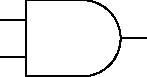
\includegraphics{Images/And.pdf }
				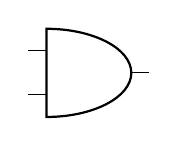
\begin{tikzpicture}
					\node at (0,0) [and port]{};
				\end{tikzpicture}
			\end{center}
			\caption{\textit{AND}}
		\end{subfigure}
		\begin{subfigure}[c]{0.3\textwidth}
			\begin{center}
				%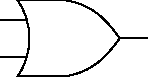
\includegraphics{Images/Or.pdf }
				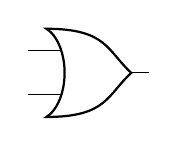
\begin{tikzpicture}
					\node at (0,0) [or port]{};
				\end{tikzpicture}
			\end{center}
			\caption{\textit{OR}}
		\end{subfigure}
		\begin{subfigure}[c]{0.3\textwidth}
			\begin{center}
				%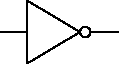
\includegraphics{Images/Not.pdf }
				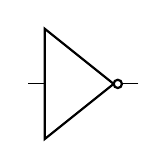
\begin{tikzpicture}
					\node at (0,0) [not port]{};
				\end{tikzpicture}
			\end{center}
			\caption{\textit{NOT}}
		\end{subfigure}
	\end{center}
	\caption{Porte logiche and, or e not}
\end{figure}
\subsection{Circuiti combinatori}
\subsubsection*{Decoder}
Ad ogni combinazione di input si associa accende un solo output. Vediamo un esempio di un decode con ingresso a 3 bit
%\vskip3mm
%\begin{minipage}[c]{0.48\textwidth}
% 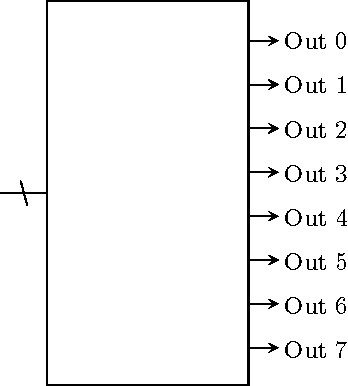
\includegraphics{Images/Decoder.pdf }
%\end{minipage}
%\vskip3mm
\vskip3mm
\begin{minipage}[c]{0.48\textwidth}
	\begin{tikzpicture}
		\draw (0,0)|-(4, -8)|-(0,0) ;
		\draw (0,-4)--++(-0.5, 0) ++ (0.25, 0) node {$/$};
		%\foreach \x/\y in {{-8/9}/cA,{-16/9}/cB, {-24/9}/cD,{-32/9}/cE,{-40/9}/cF,{-48/9}/cG,{-56/9}/cH,{-64/9}/cI}{
		%  \draw (\y) at (4, \x);
		% };
		\foreach \x [parse = true] in {-8/9, -16/9,..., -7.9}{
				\draw [-latex](4,\x) --++(0.5,0);
			}
		\foreach \x [parse = true] in {-8/9, -16/9,..., -7.9}{
				\draw [-latex](4,\x) --++(0.5,0);
			}
		\foreach \x/\y [parse = true] in {{-8/9}/1,{-16/9}/2,{-24/9}/3,{-32/9}/4,{-40/9}/5,{-48/9}/6,{-56/9}/7,{-64/9}/8}{
				\node [anchor = west] at (4.5, \x) {Out \y};
			}
	\end{tikzpicture}
\end{minipage}
%
\begin{minipage}[c]{0.48\textwidth}
	Il dispositivo qui a sinistra prende 3 input e, per ogni input, vi sarà solo uno degli 8 output che si attiveranno
\end{minipage}
\begin{center}
	\begin{tabular}{|ccc|cccccccc|}
		\hline \multicolumn{3}{|c|}{ Inputs } & \multicolumn{8}{c|}{ Outputs }                                                               \\
		\hline In2                            & In1                            & Ino & Out7 & Out6 & Out5 & Out4 & Out3 & Out2 & Out1 & Out0 \\
		0                                     & 0                              & 0   & 0    & 0    & 0    & 0    & 0    & 0    & 0    & 1    \\
		0                                     & 0                              & 1   & 0    & 0    & 0    & 0    & 0    & 0    & 1    & 0    \\
		0                                     & 1                              & 0   & 0    & 0    & 0    & 0    & 0    & 1    & 0    & 0    \\
		0                                     & 1                              & 1   & 0    & 0    & 0    & 0    & 1    & 0    & 0    & 0    \\
		1                                     & 0                              & 0   & 0    & 0    & 0    & 1    & 0    & 0    & 0    & 0    \\
		1                                     & 0                              & 1   & 0    & 0    & 1    & 0    & 0    & 0    & 0    & 0    \\
		1                                     & 1                              & 0   & 0    & 1    & 0    & 0    & 0    & 0    & 0    & 0    \\
		1                                     & 1                              & 1   & 1    & 0    & 0    & 0    & 0    & 0    & 0    & 0    \\
		\hline
	\end{tabular}
\end{center}
\subsubsection*{Multiplexer}
%\begin{minipage}[c]{0.48\textwidth}
%  \begin{figure}[H]
%    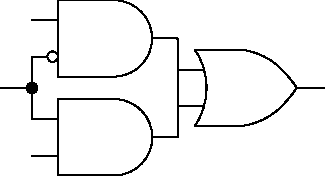
\includegraphics{Images/Multiplexer.pdf }
%  \end{figure}
%\end{minipage}
\begin{minipage}[c]{0.48\textwidth}
	\begin{tikzpicture}
		\node (A)[and port] at(0,0) {};
		\node (B)[and port] at(0,-1.5) {};
		\draw (A.in 2)--(B.in 1);
		\node (M)[blackdot] at ($(A.in 2)!0.5!(B.in 1)$){};
		\draw (M)--++(-0.5,0);
		\node (C) [anchor = west, or port] at ($(A.out)!0.5!(B.out)$){};
		\draw (A.out)--(C.in 1);
		\draw (B.out)--(C.in 2);
		\node [whitedot,anchor = east] at (A.bin 2) {};
	\end{tikzpicture}
\end{minipage}
%
\begin{minipage}[c]{0.48\textwidth}
	Il multiplexer è un dispositivo che funziona come una leva selettrice. Dati due input ed un terzo di selezione permette di dare in output uno dei due in base al valore del inout selettore
\end{minipage}
\subsubsection*{Multiplexer a più vie}
Un multiplexer può essere un selettore a molteplici ingressi. Questo fa uso di un decoder
%\begin{center}
% \includegraphics{Images/Multiplexer_più_vie.pdf }
%\end{center}
\begin{tikzpicture}

\end{tikzpicture}
\begin{figure}[H]
	\begin{center}
		\begin{tikzpicture}
			\draw (0,0) |- (4, -8) |- (0,0);
			\draw (0,-4) --++ (-0.5, 0) ++ (0.25, 0) node {$/$};
			\foreach \x/\y [parse=true] in {{-8/5}/A,{-16/5}/B,{-24/5}/C,{-32/5}/D}{
					\draw (4, \x) ++(1.5,0) node(\y) [and port, anchor = west]{};
				}
			\draw (A.in 2) -- (A.in 2 -| 4,0);
			\draw (B.in 2) -- (B.in 2 -| 4,0);
			\draw (C.in 1) -- (C.in 1 -| 4,0);
			\draw (D.in 1) -- (D.in 1 -| 4,0);
			%
			\node [anchor = east] at (A.in 1) {In 1};
			\node [anchor = east] at (B.in 1) {In 2};
			\node [anchor = east] at (C.in 2) {In 3};
			\node [anchor = east] at (D.in 2) {In 4};
			\draw (A.out) ++ (0.5,-4/5) node(E) [or port, anchor=west]{};
			\draw (C.out) ++ (0.5,-4/5) node(F) [or port, anchor=west]{};
			\draw (A.out) -| (E.in 1);
			\draw (B.out) -| (E.in 2);
			\draw (C.out) -| (F.in 2);
			\draw (D.out) -| (F.in 1);
			\draw (E.out) ++ (0.5,-8/5) node(G) [or port, anchor=west]{};
			\draw (E.out) -| (G.in 1);
			\draw (F.out) -| (G.in 2);
		\end{tikzpicture}
	\end{center}
	\caption{Multiplexer a più vie}
\end{figure}
\subsubsection*{Programmable Logic Array (PLA)}
%\begin{minipage}[c]{0.48\textwidth}
%	\begin{center}
%		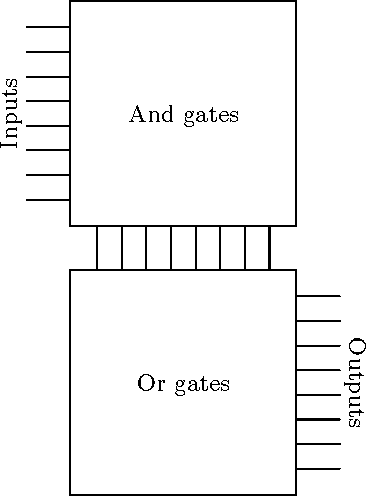
\includegraphics{Images/PLA.pdf }
%	\end{center}
%\end{minipage}
%
\begin{minipage}[c]{0.48\textwidth}
	\begin{tikzpicture}
		\draw (0,0) -| (4,-4) -| cycle;
		\node (And gates)at (2,-2) {And gates};
		\draw (0,-4/9)
		\foreach \x in {1,...,8}{
				--++(-4/9,0) ++ ( 4/9, -4/9)
			};
		\draw (4/9, -4)
		\foreach \x in {1,...,8}{
				--++(0,-4/9) ++ ( 4/9,4/9 )
			};
		\draw (0,-4-4/9) -|++ (4,-4) -| cycle;
		\draw (4+4/9,-4-8/9)
		\foreach \x in {1,...,8}{
				--++(-4/9,0) ++ ( 4/9, -4/9)
			};
		\node (Or gates) at (2,-4-4/9-2) {Or gates};
		\node [rotate = 90, anchor = south] at ([shift={(-2 - 4/9,0)}]And gates) {Inputs};
		\node [rotate = -90, anchor = south] at ([shift={(2 + 4/9,0)}]Or gates) {Outputs};
	\end{tikzpicture}
\end{minipage}
\begin{minipage}[c]{0.48\textwidth}
	Come visto in \textit{sezione} \ref{RappRetiLogiche}, possiamo convertire qualsiasi espressione da da una tabella logica ad un'espressione booleana seguendo il principio di \textit{forma canonica SP}, ossia utilizzando una serie di \textit{or} fra gruppi di \textit{and}. Lo stesso procedimento può essere applicato alle porte logiche come riportato a sinistra.
\end{minipage}
\vskip3mm
Vediamo un esempio. Cerchiamo di rappresentare le seguenti espressioni tramite un \textit{PLA}:
\begin{align*}
	D & =A+B+C                                                                                        \\
	F & =A \cdot B \cdot C                                                                            \\
	E & =(A \cdot B \cdot \overline{C})+(A \cdot C \cdot \overline{B})+(B \cdot C \cdot \overline{A})
\end{align*}
In questo caso potrei rappresentare queste espressioni tramite il seguente circuito:
%\begin{center}
%	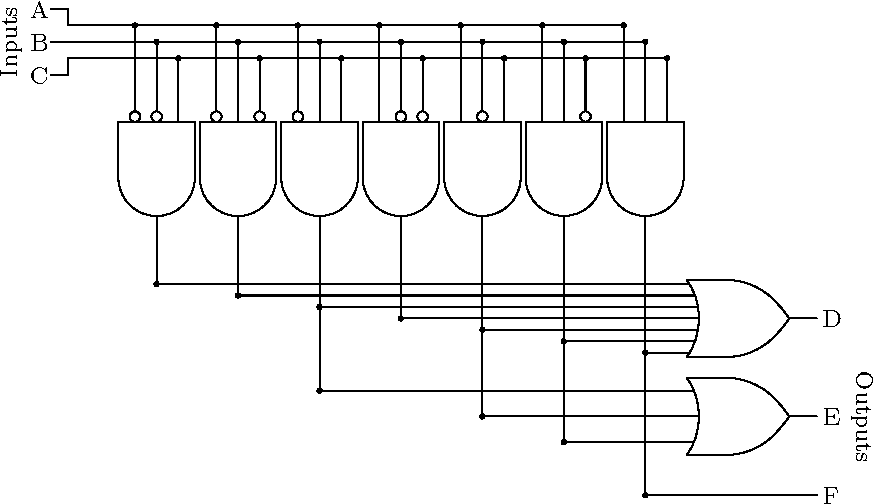
\includegraphics{Images/PLA_schemi.pdf }
%\end{center}
\vskip3mm
\begin{tikzpicture}
	\draw \foreach \x in {A,...,G}{
			node [and port, number inputs = 3, rotate = -90](\x){} ++ (1.5,0)
		};
	\node [or port, number inputs = 7, anchor = west](AND1) at (G.north|-0,-1){};
	\node [or port, number inputs = 3, anchor = west](AND2) at (G.north|-0,-2.5){};
	\node [inner sep = 0pt](AND3) at ([shift={(0,-1)}]AND2.east){};
	%
	\foreach \x/\y in {1/A, 2/B, 3/C, 4/D, 5/E, 6/F, 7/G}{
			\draw (\y.out) to[short, -*] (\y |- AND1.in \x) -- (AND1.in \x);
		}
	\foreach \x/\y in {1/C, 2/E, 3/F}{
			\draw (\y.out) to[short, -*] (\y |- AND2.in \x) -- (AND2.in \x);
		}
	\draw (G) to[short, -*] (G|-AND3) -- (AND3) {};
	\foreach \x in {A,...,G}{
			\draw (\x.in 1) to [short, -*] ([shift={(0,0.2)}]\x.in 1);
			\draw (\x.in 2) to [short, -*] ([shift={(0,0.4)}]\x.in 2);
			\draw (\x.in 3) to [short, -*] ([shift={(0,0.6)}]\x.in 3);
		}
	\draw ([shift={(0,0.2)}]G.in 1) -- ([shift={(0,0.2)}]G.in 1 -| -2,0);
	\draw ([shift={(0,0.4)}]G.in 2) -- ([shift={(0,0.4)}]G.in 1 -| -2,0);
	\draw ([shift={(0,0.6)}]G.in 3) -- ([shift={(0,0.6)}]G.in 1 -| -2,0);
	%
	\node (a)at ([shift={(-0.5,0.8)}]G.in 1 -| -2,0) {A};
	\node (b)at ([shift={(-0.5,0.4)}]G.in 1 -| -2,0) {B};
	\node (c)at ([shift={(-0.5,0)}]G.in 1 -| -2,0) {C};
	%
	\draw (a)-| ([shift={(0,0.6)}]G.in 1 -| -2,0);
	\draw (b)-| ([shift={(0,0.4)}]G.in 1 -| -2,0);
	\draw (c)-| ([shift={(0,0.2)}]G.in 1 -| -2,0);
	\node [rotate = 90, anchor = south] at (b.west){Inputs};
	\node [anchor = west] at (AND1.east){D};
	\node (letter e)[anchor = west] at (AND2.east){E};
	\node [anchor = west] at (AND3.east){F};
	%
	\node [whitedot, anchor = south] at ({A.bin 3}){};
	\node [whitedot, anchor = south] at ({A.bin 2}){};
	\node [whitedot, anchor = south] at ({B.bin 3}){};
	\node [whitedot, anchor = south] at ({B.bin 1}){};
	\node [whitedot, anchor = south] at ({C.bin 1}){};
	\node [whitedot, anchor = south] at ({D.bin 1}){};
	\node [whitedot, anchor = south] at ({D.bin 2}){};
	\node [whitedot, anchor = south] at ({E.bin 2}){};
	\node [whitedot, anchor = south] at ({F.bin 1}){};
	\node [anchor = south, rotate=-90] at (letter e.east){Outputs};
\end{tikzpicture}
\subsection{Costo e ottimizzazione operazioni}
Chiaramente per massimizzare l'efficienza è opportuno ridurre al minimo il numero di operazioni da effettuare. Per fare ciò possiamo applicare l'algebra di boole, ad esempio
\[
	\begin{aligned}
		f\left(x_1, x_2, x_3\right) & =\bar{x}_1 \bar{x}_2 \bar{x}_3+\bar{x}_1 \bar{x}_2 x_3+x_1 \bar{x}_2 \bar{x}_3+x_1 \bar{x}_2 x_3 \\
		                            & =\bar{x}_1 \bar{x}_2\left(\bar{x}_3+x_3\right)+x_1 \bar{x}_2\left(\bar{x}_3+x 3\right)           \\
		                            & =\bar{x}_1 \bar{x}_2+x_1 \bar{x}_2                                                               \\
		                            & =\left(\bar{x}_1+x_1\right) \bar{x}_2                                                            \\
		                            & =\bar{x}_2
	\end{aligned}
\]
tuttavia la semplificazione delle reti logiche non è sempre una mansione semplice. Talvolta ci si basa sull'applicazione iterativa delle regole dell'\textit{algebra di boole}, per casi semplici ci si appooggia a metodi grafici (\textit{mappe di Karnaugh}). Questo topic è approfondito nel corso \underline{Reti Logiche}
\subsection{Circuiti sequenziali}
I \underline{circuiti sequenziali} sono necessari l'addove viene introdotto qualche meccanismo in grado di \underline{memorizzare} dei dati. Tale memorizzazione avviene tramite un meccanismo di \underline{retrorotazione}, ossia reindirizzando l'uscita del circuito all'entrata del circuito stesso. Vediamo un esempio:
\subsubsection*{R-S Latch}

%\begin{figure}[H]
%	\begin{center}
%		\begin{subfigure}[c]{0.45\textwidth}
%			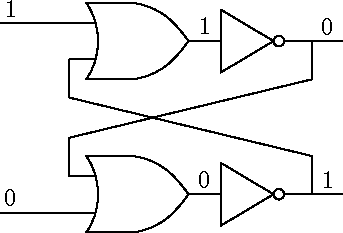
\includegraphics{Images/RS_latch1.pdf}
%			\caption{Set}
%		\end{subfigure}
%		\begin{subfigure}[c]{0.45\textwidth}
%			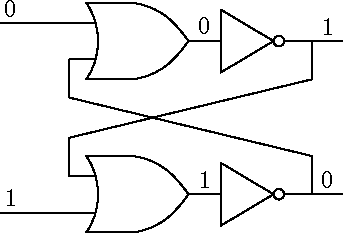
\includegraphics{Images/RS_latch2.pdf}
%			\caption{Reset}
%		\end{subfigure}
%	\end{center}
%\end{figure}
\begin{figure}[H]
	\begin{subfigure}[c]{0.45\textwidth}
		\begin{center}
			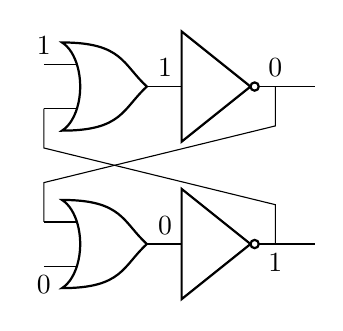
\begin{tikzpicture}
				\draw (0,1) node(A) [anchor = east, or port]{};
				\node (B)[anchor = west, not port] at (A.east){};
				\node (q)[anchor = south] at (B.out){0};
				\draw (B.east) -- ++(0.5,0);
				%
				\draw (0,-1) node(C) [anchor = east, or port, number inputs=2]{};
				\node (D)[anchor = west, not port] at (C.east){};
				\node (q)[anchor = north] at (D.out){1};
				\draw (D.east) -- ++(0.5,0);
				%
				\draw (B.east) -- ++(0,-0.5) -- ([shift={(0,0.5)}]C.in 1) -- (C.in 1);
				\draw (A.in 2) -- ++(0, -0.5) -- ([shift = {(0,0.5)}]D.east) --++ (0,-0.5);;
				\node [anchor = south] at (A.in 1){1};
				\node [anchor = north] at (C.in 2){0};
				\node [anchor = south] at (A.out){$1$};
				\node [anchor = south] at (C.out){$0$};
			\end{tikzpicture}
		\end{center}
		\caption{Set}
	\end{subfigure}
	\begin{subfigure}[c]{0.45\textwidth}
		\begin{center}
			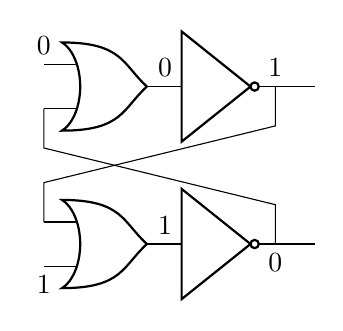
\begin{tikzpicture}
				\draw (0,1) node(A) [anchor = east, or port]{};
				\node (B)[anchor = west, not port] at (A.east){};
				\node (q)[anchor = south] at (B.out){1};
				\draw (B.east) -- ++(0.5,0);
				%
				\draw (0,-1) node(C) [anchor = east, or port, number inputs=2]{};
				\node (D)[anchor = west, not port] at (C.east){};
				\node (q)[anchor = north] at (D.out){0};
				\draw (D.east) -- ++(0.5,0);
				%
				\draw (B.east) -- ++(0,-0.5) -- ([shift={(0,0.5)}]C.in 1) -- (C.in 1);
				\draw (A.in 2) -- ++(0, -0.5) -- ([shift = {(0,0.5)}]D.east) --++ (0,-0.5);;
				\node [anchor = south] at (A.in 1){0};
				\node [anchor = north] at (C.in 2){1};
				\node [anchor = south] at (A.out){0};
				\node [anchor = south] at (C.out){1};
			\end{tikzpicture}
		\end{center}
		\caption{Reset}
	\end{subfigure}
\end{figure}
Nelle operazioni di reset e set nota che:
\begin{itemize}
	\item La porta or che vede come input un 1 chiaramente avrà come output 1, che negato diventerà 0
	\item Lo 0 verra retropropagato alla porta or con ingresso 0 che darà come out 0, che negato diventerà 1
	\item Abbiamo ottenuto così una situazione stabile
\end{itemize}
Chiaramente il discorso vale anche per l'operazione di reset. Diverso è il discorso per l'operazione di store
%\begin{center}
%	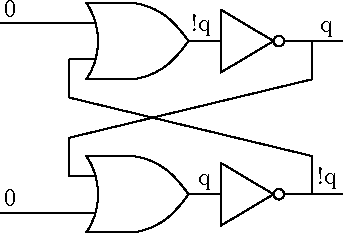
\includegraphics{Images/RS_latch3.pdf }
%\end{center}
\begin{center}
	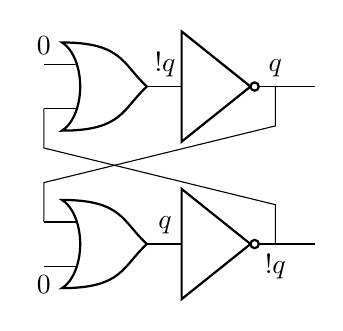
\begin{tikzpicture}
		\draw (0,1) node(A) [anchor = east, or port]{};
		\node (B)[anchor = west, not port] at (A.east){};
		\node (q)[anchor = south] at (B.out){$q$};
		\draw (B.east) -- ++(0.5,0);
		%
		\draw (0,-1) node(C) [anchor = east, or port, number inputs=2]{};
		\node (D)[anchor = west, not port] at (C.east){};
		\node (q)[anchor = north] at (D.out){$!q$};
		\draw (D.east) -- ++(0.5,0);
		%
		\draw (B.east) -- ++(0,-0.5) -- ([shift={(0,0.5)}]C.in 1) -- (C.in 1);
		\draw (A.in 2) -- ++(0, -0.5) -- ([shift = {(0,0.5)}]D.east) --++ (0,-0.5);;
		\node [anchor = south] at (A.in 1){0};
		\node [anchor = north] at (C.in 2){0};
		\node [anchor = south] at (A.out){$!q$};
		\node [anchor = south] at (C.out){$q$};
	\end{tikzpicture}
\end{center}
\vskip3mm
In questo caso la situazioe è la seguente:
\begin{itemize}
	\item Suppiniamo di fare un fermaimmagine e cambiare improvvismente l'input alle porte or
	\item Avendo una porta or con un'estremità uguale a 0 l'output coinciderà con l'input proveniente dalla porta non nulla
	\item Otteniamo così anche qui una situazione stabile: supponendo di avere un segnale di tipo $ q $ e $ !q $ in uscita dalle porte \textit{or} finchè verra dato in ingresso 0 ad entrambe si avrà in uscita sempre $ q $ e $ !q $
\end{itemize}
\textbox{NB: se si fornisce 1 ad entrambe le porte \textit{or} il circuito entrerebbe in uno stato \underline{indeterministico}. Ciò vuol dire che non è possibile stabilire l'output del circuito}
\subsubsection*{Clock}
Per negare la possibilità di effettuare operazioni di \textit{set} e \textit{reset} in determinati momenti è possibile aggiungere un terzo input al \textit{R-S Latch}:
%\begin{center}
%	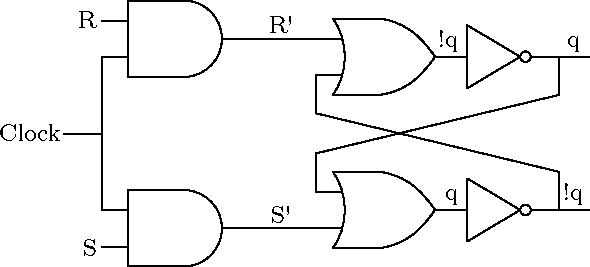
\includegraphics{Images/Clock.pdf}
%\end{center}
\begin{center}
	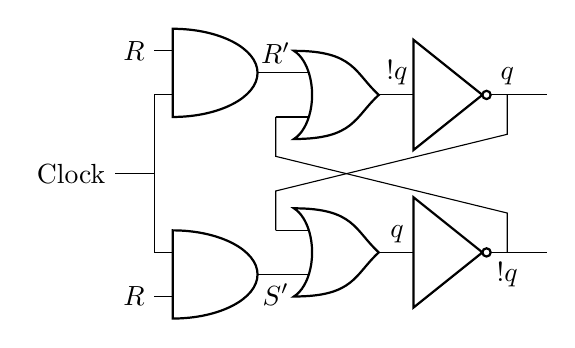
\begin{tikzpicture}
		\draw (0,1) node(A) [anchor = east, or port]{};
		\node (B)[anchor = west, not port] at (A.east){};
		\node (q)[anchor = south] at (B.out){$q$};
		\draw (B.east) -- ++(0.5,0);
		%
		\draw (0,-1) node(C) [anchor = east, or port, number inputs=2]{};
		\node (D)[anchor = west, not port] at (C.east){};
		\node (q)[anchor = north] at (D.out){$!q$};
		\draw (D.east) -- ++(0.5,0);
		%
		\draw (B.east) -- ++(0,-0.5) -- ([shift={(0,0.5)}]C.in 1) -- (C.in 1);
		\draw (A.in 2) -- ++(0, -0.5) -- ([shift = {(0,0.5)}]D.east) --++ (0,-0.5);;
		\node [anchor = south] at (A.in 1){$R'$};
		\node [anchor = north] at (C.in 2){$S'$};
		\node [anchor = south] at (A.out){$!q$};
		\node [anchor = south] at (C.out){$q$};
		\node (E)[and port, anchor = east] at (A.in 1) {};
		\node (F)[and port, anchor = east] at (C.in 2) {};
		\node [anchor = east] at (E.in 1) {$R$};
		\node [anchor = east] at (F.in 2) {$R$};
		\draw (E.in 2)--(F.in 1);
		\draw ($(E.in 2)!0.5!(F.in 1)$) --++(-0.5,0) node [anchor = east] {Clock};
	\end{tikzpicture}
\end{center}
In questo caso se il clock è 0 non possono avvenire transizioni di stato (stato \textit{no change}). Se invece il clock vale 1 è come se le due porte \textit{and} non esistano, ed il circuito funziona come spiegato sopra
\subsubsection*{D-Latch}
Per risolvere il problema del possibile input di due 1 in un \textit{R-S Latch} un input di \underline{clock}. Il circuito è il seguente:
%\begin{center}
%	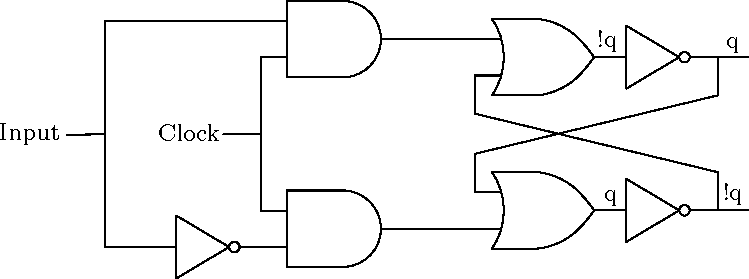
\includegraphics{Images/D_latch.pdf }
%\end{center}
\begin{center}
	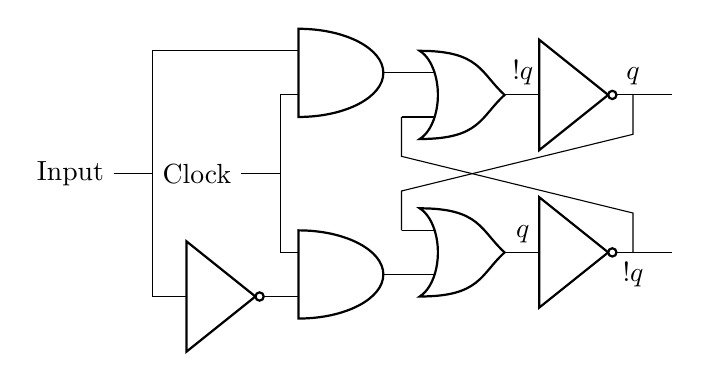
\begin{tikzpicture}
		\draw (0,1) node(A) [anchor = east, or port]{};
		\node (B)[anchor = west, not port] at (A.east){};
		\node (q)[anchor = south] at (B.out){$q$};
		\draw (B.east) -- ++(0.5,0);
		%
		\draw (0,-1) node(C) [anchor = east, or port, number inputs=2]{};
		\node (D)[anchor = west, not port] at (C.east){};
		\node (q)[anchor = north] at (D.out){$!q$};
		\draw (D.east) -- ++(0.5,0);
		%
		\draw (B.east) -- ++(0,-0.5) -- ([shift={(0,0.5)}]C.in 1) -- (C.in 1);
		\draw (A.in 2) -- ++(0, -0.5) -- ([shift = {(0,0.5)}]D.east) --++ (0,-0.5);;
		\node [anchor = south] at (A.out){$!q$};
		\node [anchor = south] at (C.out){$q$};
		\node (E)[and port, anchor = east] at (A.in 1) {};
		\node (F)[and port, anchor = east] at (C.in 2) {};
		\draw (E.in 2)--(F.in 1);
		\draw ($(E.in 2)!0.5!(F.in 1)$) --++(-0.5,0) node (clock) [anchor = east] {Clock};
		\node (input) [anchor = east] at ([shift={(-0.5, 0)}] clock.west) {Input};
		\draw (input.east) --++ (0.5, 0) |- (E.in 1);
		\node [not port, anchor = east] (notport) at (F.in 2) {};
		\draw (input.east) --++ (0.5, 0) |- (notport.in);
		%\draw (input) --++ (0.5, 0) |- (E.in 1);
	\end{tikzpicture}
\end{center}
Negando uno dei due ingressi non è possibile che si presenti il caso in cui entrambi siano 1. L'operazione di \textit{store}(che richiede entrambi gli input nulli) verrà effettuata solo tramite il \underline{clock}
\subsubsection*{Rappresentazione compatta latch}
Visto che questi componenti sono estremamente comuni, si possono rappresentare in versone compatta come segue, all'interno di un circuito:
\begin{figure}[H]
	\begin{center}
		\begin{subfigure}{0.3\textwidth}
			\begin{center}
				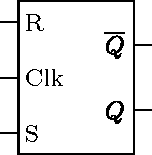
\includegraphics{Images/RS_latch_compatta.pdf}
				\caption{RS\_latch}
			\end{center}
		\end{subfigure}
		\begin{subfigure}{0.3\textwidth}
			\begin{center}
				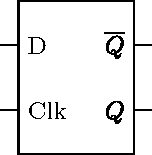
\includegraphics{Images/D_latch_compatta.pdf}
				\caption{D\_latch}
			\end{center}
		\end{subfigure}
		\begin{subfigure}{0.3\textwidth}
			\begin{center}
				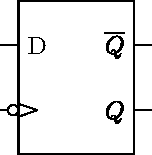
\includegraphics{Images/Flip_flop_master_slave.pdf}
				\caption{Flip Flop Master Slave}
			\end{center}
		\end{subfigure}
	\end{center}
	\caption{Rappresentazione simbolica latch}
\end{figure}
\subsubsection*{Flip Flop master-slave}
Questo tipo di \textit{latch} permette di effettuare la memorizzazione esattamente alla fine del ciclo di clock. Il circuito è il seguente:
\begin{center}
	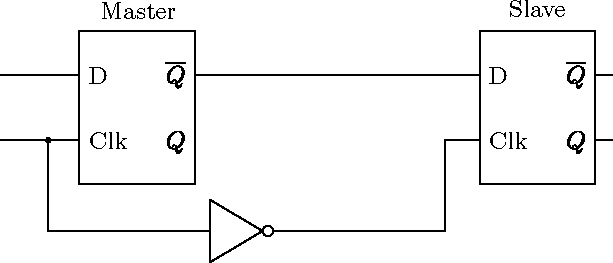
\includegraphics{Images/Flip_flop_master_slave_circuito.pdf }
\end{center}
In questo caso abbiamo che:
\begin{itemize}
	\item Se il \textit{clock} è 1 allora il latch \textit{slave} è "inattivo" (stato di \textit{store}), mentre \textit{master} sarà sensibile a \textit{set} e \textit{reset}
	\item Se il \textit{clock} è 0 allora \textit{master} memorizzerà lo stato e setterà il latch \textit{slave} si conseguenza
	\item In quessto caso quindi, la memorizzazione avviene quando il clock diventa 0
\end{itemize}
\section{Terminologia e definizioni}
\subsubsection*{Funzionamento cpu}
Ogni processore è in grado di comunicare solo fornendo in ingresso delle stringhe di dati, che possiedono una data codifica la quale cambia da cpu a cpu. In particolare una cpu funziona nel modo seguente:
\begin{itemize}
	\item \textit{Fetch} l'istruzione da eseguire viene prelevata dalla memoria. Esiste un particolare registro (\underline{Program Counter PC/ Instructions Pointer (IP)})
	\item \textit{Decode} l'istruzione (stringa di byte) viene decodificata
	\item \textit{Execute} l'istruzione decodificata viene eseguita
\end{itemize}
Il linguaggio assembly permette di chiamare queste procedure rese possibili dalla cpu, seza scrivere codice  binario. Ogni qualvolta si chiami una procedura assembly questa viene mappata dunque in una stringa di bit (solitamente 32)

\subsubsection*{Registri}
Un registro non è altro che un'area di memoria vicino al processore ad accesso rapido. Quest'area è composta da batterie di registri flip flop di tipo D ($ k $ registri per $ k $ byte). In genere sono presenti dai 4 ai 64 registri
\subsubsection*{Macchina a 32/64 bit}
Quando si dice che una macchina è a \textit{x} bit si intende che i registri di questa hanno tutti dimensione \textit{x} bit
\subsubsection*{Instructions Set Architecture}
L'Instruction Set Architecture è l'insieme di regole per interfacciarsi con una determinata cpu. In poche parole sono le stringhe di bit che sono interpretaili da una cpu. Le seguenti cose sono definite all'interno dell'isa di una cpu:
\begin{itemize}
	\item Sintassi e semantica
	\item Istruzioni disponibili
	\item Numero di registri, tipo e dimensione
	\item Modalità di accesso alla memoria (\textit{indirizzamento})
	\item Istruzioni assembly disponibili
\end{itemize}
Alcuni registri sono messi a disposizione per eseguire e memorizzarci temporaneamente dati (i cosiddetti registri \textit{general-purpose}) da parte dell'utente, mentre altri sono riservati e contengono dati specifici
\vskip3mm
Esistono 3 macrocategorie di ISA:
\begin{itemize}
	\item \textit{RISC} Reduced Instruction Set Computer
	      \begin{itemize}
		      \item Semplice e regolare
		      \item Istruzioni lavorano su registri e non su memoria direttamente
		      \item Accesso alla memoria solo tramite 2 istruzioni: \textit{load} e \textit{store}
		      \item Molte meno istruzioni e meno potenti
		      \item Cpu molto più facile da costruire
	      \end{itemize}
	\item \textit{CISC} Complex Instruction Set Computer
	      \begin{itemize}
		      \item Molte più istruzioni più complesse e più potenti
		      \item Ogni istruzione può accedere ai registri o direttamente alla memoria
	      \end{itemize}
	\item \textit{ARM} Advanced RISC Machine
	      \begin{itemize}
		      \item Via di mezzo fra RISC e CISC.
	      \end{itemize}
\end{itemize}
\subsubsection*{Application Binary Interface (ABI)}
Le modalità di uso dei registri non è spesso imposta dall'hardware. Per questa ragione esistono le \textit{ABI}, ossia convenzioni software circa l'uso dei registri. Le \textit{convenzioni di chiamata} ne sono un esempio.Ad esempio le convenzioni di chiamata specificatno
\begin{itemize}
	\item Come / dove passare i parametri ad una subroutine/funzione
	\item Quali registri vanno preservati nel momento in cui si chiama una funzione
	\item Quali registri conterranno il valore di ritorno di una data funzione
\end{itemize}
\subsubsection*{Accesso alla memoria}
\begin{minipage}[c]{0.30\textwidth}
	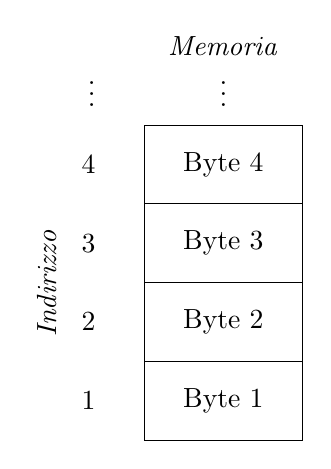
\begin{tikzpicture}
		\draw (0,0)|-(2, -4) |- (0,0);
		\draw (0,-1)--++(2,0);
		\draw (0,-2)--++(2,0);
		\draw (0,-3)--++(2,0);
		\draw (0,-4)--++(2,0);
		\node at (1, -0.5) {Byte 4};
		\node at (1, -1.5) {Byte 3};
		\node at (1, -2.5) {Byte 2};
		\node at (1, -3.5) {Byte 1};
		\node [anchor = east] at (-0.5, -0.5) {4};
		\node [anchor = east] at (-0.5, -1.5) {3};
		\node [anchor = east] at (-0.5, -2.5) {2};
		\node [anchor = east] at (-0.5, -3.5) {1};
		\node at (1, 1) {\textit{Memoria}};
		\node at (1, 0.5) {$\vdots$};
		\node [anchor = east] at (-0.5, 0.5) {$\vdots$};
		\node [anchor = south, rotate = 90] at (-1, -2) {\textit{Indirizzo}};
	\end{tikzpicture}
\end{minipage}
%
\begin{minipage}[c]{0.65\textwidth}
	La memoria di una macchina è indicizzata: ci si può riferire ad ogni zona della memoria ram specificando un numero. Questo numero viene detto \textit{indirizzo}. La memoria è suddivisa in gruppi da 8 bit, ossia in gruppi di \textit{byte}. L'indizirro incrementa di 1 per ongi byte
\end{minipage}
\vskip3mm
L'accesso alla memoria può avvenire secondo diverse modalità
\begin{itemize}
	\item \textit{Indirizzo assoluto}: l'indirizzo di memoria viene indicato all'interno dell'istruzione stessa. Questo può comportare problemi se nell'architettura le istruzioni hanno larghezza costante (ad esempio 32 bit), in quanto il numero dell'indirizzo può essere troppo grande
	\item \textit{Indiretto}: l'indirizzo è contenuto all'interno di un registro indicato nell'istruzione stessa
	\item \textit{Base + spiazzamento}: indirizzo è ottenuto sommando un valore costante (immediato) ad un indirizzo contenuto in un registro
	\item \textit{Base + indice}: Simile al metodo precedente, tuttavia anziché usare un valore costante si utilizza un altro registro contenente il valore di spiazzamento
	\item Simile al metodo precedente, con la possibilità di aggiungere anche un valore costante
\end{itemize}
\textbox{In alcune ISA è presente il cosidetto \underline{vincolo di allineamento}, ossia è possibile accedere solo a indirizzi multipli di 8 o 4 byte. Ciò è sensato visto che i dati manipolati sono quasi sempre stringhe di 64 p 32 bit}
\section{Assembly Risc-V}
L'ISA Risc-V ha la caratteristica di essere \underline{modulare}. Ciò vuol dire che il produttore di ciascun chip può decidere di implementare o meno date funzionalità. Tali funzionalità vengono dette \underline{estensioni}. Le estenzioni che un chip implementa sono specificate da una sigla, nel seguente formato:
\begin{center}
	\begin{tikzpicture}
		\node (a)at (0,0) {\verb|rv|};
		\node (b)[anchor = west] at (a.east) {\verb|32/64/128|};
		\node (c)[anchor = west] at (b.east) {\verb|MAFDQLCBTPV|};
		\draw [dashed] (b.north west)--(c.north east)|-(b.south west)-- (b.north west);
		\draw [dashed] (c.north west)--(c.south west);
		\node [fit = (a) (b) (c), draw] {};
		\draw [dashed](b.south)|-++(-0.8,-0.4)--++(0,-0.2)node [anchor = north] {Architettura a \textit{x} bit};
		\draw [dashed](c.south)|-++(0.8,-0.4)--++(0,-0.2) node [anchor = north] {Estensioni incluse};
	\end{tikzpicture}
\end{center}
Le estensioni più comuni sono le seguenti:
\begin{itemize}
	\item \underline{RV32I} \textit{Base Integer Instruction Set} implementa tutte le funzionalità di base. Ogni ISA Risc-V deve necessariamente implementare almeno questa estensione
	\item \underline{RV32M}\textit{Standard Extension for Integer Multiplication and Division} implementa funzioni quali \verb|div| o \verb|mul|
	\item \underline{RV32F} \textit{Standard Extension for Single-Precision Floating-Point} permette di lavorare su numeri con la virgola
	\item \underline{RV32G} \textit{General Purpose scalar Instruction Set} implementa tutte le seguenti estensioni: \textit{IMAFD}
	      i
\end{itemize}
\subsection{Istruzioni base RV64I}
\subsubsection*{Istruzioni aritmetiche}
\command{add}{dest reg1 reg2}{}{somma le variabili \textit{reg1} e \textit{reg2} salvandole in \textit{dest}}
\command{sub}{dest reg1 reg2}{prova}{sottrae \textit{reg2} a \textit{reg1}, salvando in \textit{dest}}
\subsubsection*{Accesso alla memoria}
\command{lw}{dest x(base)}{}{carica la word situata in $ base + x $ ($ x $ espresso in byte) in \textit{dest}}
\command{sw}{dest x(base)}{}{salva la word situata in $ base + x $ ($ x $ espresso in byte) in \textit{dest}}
\command{ld}{dest x(base)}{}{carica la double word situata in $ base + x $ ($ x $ espresso in byte) in \textit{dest}}
\command{sd}{dest x(base)}{}{salva la double word situata in $ base + x $ ($ x $ espresso in byte) in \textit{dest}}
\subsubsection*{Operatori logici}
\command{and}{dest reg1 reg2}{}{effettua l'\textit{and} bit a bit fra \textit{reg1} e \textit{reg2}, salvando il risultato in \textit{dest}}
\command{or}{dest reg1 reg2}{}{effettua l'\textit{or} bit a bit fra \textit{reg1} e \textit{reg2}, salvando il risultato in \textit{dest}}
\command{xor}{dest reg1 reg2}{}{effettua lo \textit{xor} bit a bit fra \textit{reg1} e \textit{reg2}, salvando il risultato in \textit{dest}}
Lo \textit{xor} restituisce 1 se entrambi i numeri sono diversi, altrimenti 0. Ha 2 use cases:
\begin{itemize}
	\item Ottenere  0x000  effettuando lo \textit{xor} con se stesso
	\item Applicare il negato, effettuando lo \textit{xor} con tutti uni
\end{itemize}
\subsubsection*{Operazioni di shifting}
Lo shift è importantissimo in quanto shiftare un numero a sinistra/destra corrisponde alla moltiplicazione/divisione per una potenza di 2
\command{slli}{dest reg1, ammount}{}{shifta di \textit{ammount} posizioni sinistra il numero contenuno in \textit{reg1} e lo salva in \textit{dest}}
Nota che se si applica lo shift a sinistra a determinati numeri si ottiene on overflow, ad esempio:
\begin{center}
	\begin{footnotesize}
		\begin{tabular}{|c c c c c c c c|}
			\hline
			10000000 & 00000000 & 00000000 & 00000000 & 00000000 & 00000000 & 00000000 & 00000001 \\
			\hline
		\end{tabular}
  \end{footnotesize}%\command{cd}{"path"}{}{current directory} 
\end{center}
\command{srli}{dest reg1, ammount}{}{shifta di \textit{ammount} posizioni a destra il numero contenuno in \textit{reg1} e lo salva in \textit{dest}}
Allo stesso modo, anche uqesto shift può dare peroblemi di overflow, ad esempio:
\begin{center}
	\begin{footnotesize}
		\begin{tabular}{|c c c c c c c c|}
			\hline
			11111111 & 11111111 & 00000000 & 00000000 & 00000000 & 00000000 & 00000000 & 00000001 \\
			\hline
		\end{tabular}
  \end{footnotesize}%\command{cd}{"path"}{}{current directory} 
\end{center}
eseguento uno shift a destra di 4 diventerebbe:
\begin{center}
	\begin{footnotesize}
		\begin{tabular}{|c c c c c c c c|}
			\hline
			00001111 & 11111111 & 11110000 & 00000000 & 00000000 & 00000000 & 00000000 & 00000001 \\
			\hline
		\end{tabular}
  \end{footnotesize}%\command{cd}{"path"}{}{current directory} 
\end{center}
\command{srai}{dest reg1, ammount}{}{shifta di \textit{ammount} posizioni a destra il numero contenuno in \textit{reg1} e lo salva in \textit{dest}. A differenza di \textit{srli} vengono aggiunti 1 o 0 in base a quale sia la cifra più significativa}
\begin{center}
	\begin{footnotesize}
		\begin{tabular}{|c c c c c c c c|}
			\hline
			11111111 & 11111111 & 00000000 & 00000000 & 00000000 & 00000000 & 00000000 & 00000001 \\
			\hline
		\end{tabular}
  \end{footnotesize}%\command{cd}{"path"}{}{current directory} 
\end{center}
eseguento uno shift a destra aritmetico di 4 diventerebbe:
\begin{center}
	\begin{footnotesize}
		\begin{tabular}{|c c c c c c c c|}
			\hline
			11111111 & 11111111 & 11110000 & 00000000 & 00000000 & 00000000 & 00000000 & 00000001 \\
			\hline
		\end{tabular}
  \end{footnotesize}%\command{cd}{"path"}{}{current directory} 
\end{center}
\subsubsection*{Salti condizionati}
\command{beq}{reg1, reg2, L1}{}{se il contenuto del registo \textit{reg1} è uguale al registro \textit{reg2} salta all'etichetta \textit{l1}}
\command{bne}{reg1, reg2, L1}{}{se il contenuto del registo \textit{reg1} è diverso al registro \textit{reg2} salta all'etichetta \textit{l1}}
\command{blt}{reg1, reg2, L1}{}{se il contenuto del registo \textit{reg1} è minore al registro \textit{reg2} salta all'etichetta \textit{l1}}
\command{bge}{reg1, reg2, L1}{}{se il contenuto del registo \textit{reg1} è maggiore o uguale al registro \textit{reg2} salta all'etichetta \textit{l1}}
\command{bltu}{reg1, reg2, L1}{}{se il contenuto del registo \textit{reg1} è minore al registro \textit{reg2} salta all'etichetta \textit{l1}. I dati nei registri sono interpretati come dati unsigned}
\command{bgeu}{reg1, reg2, L1}{}{se il contenuto del registo \textit{reg1} è maggiore o uguale al registro \textit{reg2} salta all'etichetta \textit{l1}. I dati nei registri sono interpretati come dati unsigned}
\subsection{Procedure e convenzioni di chiamata}
\subsubsection*{Uso registri}
Nel momento in cui si chiama una funzione, sia il \textit{chiamante} che il \textit{chiamato} sono soggetti alle cosiddette \underline{convenzioni di chiamata}. Fanno parte di queste convenzioni anche regole per l'uso dei registri:
\begin{itemize}
	\item \verb|x10 - x17| vengono usati per il passaggio di parametri
	\item \verb|x1| viene usato per contenere l'\textit{indirizzo} di memoria della istruzione per ritornare al punto dal quale la funzione è stata chiamata
\end{itemize}
In particolare, i registri hanno le seguenti funzionalità:
\vskip3mm
\begin{table}[H]
	\begin{center}
		\begin{tabular}{|l|l|l|l|}
			\hline
			Register       & ABI Name       & Description                      & Saver  \\
			\hline
			\verb|x0|      & \verb| zero|   & Hard-wired zero                  & -      \\
			\verb|x1|      & \verb| ra|     & Return address                   & Caller \\
			\verb|x2|      & \verb| sp|     & Stack pointer                    & Callee \\
			\verb|x3|      & \verb| gp|     & Global pointer                   & -      \\
			\verb|x4|      & \verb| tp|     & Thread pointer                   & -      \\
			\verb|x5-7|    & \verb| t0-2|   & Temporaries                      & Caller \\
			\verb|x8|      & \verb| s0/fp|  & Saved register/frame pointer     & Callee \\
			\verb|x9|      & \verb| s1|     & Saved register                   & Callee \\
			\verb|x10-11|  & \verb| a0-1|   & Function arguments/return values & Caller \\
			\verb|x12-17|  & \verb| a2-7|   & Function arguments               & Caller \\
			\verb|x18-27|  & \verb| s2-11|  & Saved registers                  & Callee \\
			\verb|x28-31|  & \verb| t3-6|   & Temporaries                      & Caller \\
			\hline
			\verb|f0-7|    & \verb| ft0-7|  & FP temporaries                   & Caller \\
			\verb|f8-9|    & \verb| fs0-1|  & FP saved registers               & Callee \\
			\verb|f 10-11| & \verb| fa0-1|  & FP arguments/return values       & Caller \\
			\verb|f12-17|  & \verb| fa2-7|  & FP arguments                     & Caller \\
			\verb|f 18-27| & \verb| fs2-11| & FP saved registers               & Callee \\
			\verb|f28-31|  & \verb| ft8-11| & FP temporaries                   & Caller \\
			\hline
		\end{tabular}
	\end{center}
	\caption{Uso dei registri in Risc-V}
\end{table}
\begin{itemize}
	\item \verb|x1 ra| viene usato per contenere l'\textit{indirizzo} di memoria della istruzione per ritornare al punto dal quale la funzione è stata chiamata
	\item \verb|x2 sp| viene usato per contenere \textit{l'indirizzo} di memoria dell'ultimo elemento allocato sulla stack. Il prossimo indirizzo libero sarà \verb|sp-4|
	\item \verb|x3 gp| viene usato per contenere l'indirizzo della memoria statica di un programma (\textit{static segment})
	\item \verb |x8 fp| viene usato per contenere il primo indirizzo di memoria dello \textit{stack}
\end{itemize}
Le convenzioni di chiamata specificano anche un fatto importante:
\textbox{Per convenzione, alcuni registri possono essere sovrascritti durante l'esecuzione di una funzione, altri \underline{no}}
Ecco perchè nella tabella è indicato che i registri \verb|s0-s11| vanno salvati dal \textit{callee} (dalla funzione chiamata), facendo sì che al termine della procedura questi abbiano lo stesso valore che avevano \underline{prima} della chiamata, mentre i registri \verb|t0-6| possono essere usati senza essere salvati
\subsubsection*{Uso stack}
Se i registri per i parametri non dovessero bastare, è possiblie utilizzare lo stasck, tenendo in mente che:
\begin{itemize}
	\item Lo stack cresce "verso il basso". Lo stack pointer (registro \verb|sp, x2|) si sposta a valori via via più piccoli man mano che allochiamo nuovi dati sullo stack
	\item Lo stack va svuotato alla fine di cisascuna procedura
\end{itemize}
\begin{center}
	\newsavebox{\mybox}
	\begin{lrbox}{\mybox}
		\begin{tabular}{c}
			\verb| addi sp, sp, -8| \\
			\verb| ld reg y, 0(sp)| \\
			\verb| ld reg x, 4(sp)| \\
		\end{tabular}
	\end{lrbox}
	%
	\begin{tikzpicture}[scale = 0.7]
		\draw (0,0)|-(4, -8)|-(0,0);
		\draw (2,0)--(2,-8);
		\foreach \x  [parse = true] in  {-1,-2,..., -7}{
				\draw [dashed] (2, \x )--++(2,0);
			}
		\foreach \x  [parse = true] in  {-1,-2,..., -7}{
				\draw [dotted] (0, \x )--++(2,0);
			}
		\node at (1,-7.5) {\verb|0x00|};
		\node at (1,-6.5) {\verb|0x04|};
		\node at (1,-5.5) {\verb|0x08|};
		\node at (1,-4.5) {\verb|0x012|};
		\node at (1,-3.5) {\verb|0x016|};
		\node at (1,-2.5) {\verb|0x020|};
		\node at (1,-1.5) {\verb|0x024|};
		\node at (1,-0.5) {\verb|0x028|};
		\draw [-latex, shift={(-0.2,0)} ](-0.5,-0.5)node [anchor = east] {\verb|sp|} --(0,-0.5) ;
		\draw  (3,-0.5) node {\color{gray}\verb|data|};
		%
		%fig 2
		%
		\draw (6,0)|-++(4, -8)|-cycle;
		\draw (6,0)++(2,0)--++(0,-8);
		\foreach \x  [parse = true] in  {-1,-2,..., -7}{
				\draw [dashed] (6,0)++(2, \x )--++(2,0);
			}
		\foreach \x  [parse = true] in  {-1,-2,..., -7}{
				\draw [dotted] (6,0)++(0, \x )--++(2,0);
			}
		\draw (6,0) ++ (1,-7.5) node {\verb|0x00|};
		\draw (6,0) ++ (1,-6.5) node {\verb|0x04|};
		\draw (6,0) ++ (1,-5.5) node {\verb|0x08|};
		\draw (6,0) ++ (1,-4.5) node {\verb|0x012|};
		\draw (6,0) ++ (1,-3.5) node {\verb|0x016|};
		\draw (6,0) ++ (1,-2.5) node {\verb|0x020|};
		\draw (6,0) ++ (1,-1.5) node {\verb|0x024|};
		\draw (6,0) ++ (1,-0.5) node {\verb|0x028|};
		%
		\draw (6,0) ++ (3,-0.5) node {\color{gray}\verb|data|};
		\draw (6,0) ++ (3,-1.5) node {\verb|reg x|};
		\draw (6,0) ++ (3,-2.5) node {\verb|reg y|};
		\draw  [-latex, shift={(-0.2,0)} ] (6,0) ++ (-0.5,-2.5)node [anchor = east] {\verb|sp|} --++(0.5,0) ;
		%
		%fig 2
		%
		\draw (12,0)|-++(4, -8)|-cycle;
		\draw (12,0)++(2,0)--++(0,-8);
		\foreach \x  [parse = true] in  {-1,-2,..., -7}{
				\draw [dashed] (12,0)++(2, \x )--++(2,0);
			}
		\foreach \x  [parse = true] in  {-1,-2,..., -7}{
				\draw [dotted] (12,0)++(0, \x )--++(2,0);
			}
		\draw (12,0) ++ (1,-7.5) node {\verb|0x00|};
		\draw (12,0) ++ (1,-6.5) node {\verb|0x04|};
		\draw (12,0) ++ (1,-5.5) node {\verb|0x08|};
		\draw (12,0) ++ (1,-4.5) node {\verb|0x012|};
		\draw (12,0) ++ (1,-3.5) node {\verb|0x016|};
		\draw (12,0) ++ (1,-2.5) node {\verb|0x020|};
		\draw (12,0) ++ (1,-1.5) node {\verb|0x024|};
		\draw (12,0) ++ (1,-0.5) node {\verb|0x028|};
		%
		\draw (12,0) ++ (3,-0.5) node {\color{gray}\verb|data|};
		\draw (12,0) ++ (3,-1.5) node {\color{gray}\verb|reg x|};
		\draw (12,0) ++ (3,-2.5) node {\color{gray}\verb|reg y|};
		\draw  [-latex, shift={(-0.2,0)} ] (12,0) ++ (-0.5,-0.5)node [anchor = east] {\verb|sp|} --++(0.5,0) ;
		%
		%
		%
		%\draw [bend left, bend angle = 30, -latex, dotted] (2,0.2) to node [anchor = south] {\texttt{addi sp, sp, -8}}(8,0.2) ;
		\draw [bend left, bend angle = 30, -latex, dotted] (2,0.2) to node [anchor = south, draw, solid] {\usebox{\mybox}}(8,0.2) ;
		\draw [bend left, bend angle = 30, -latex, dotted] (8,0.2) to node [anchor = south, draw, solid] {\texttt{addi sp, sp, 8}}(14,0.2) ;
	\end{tikzpicture}
\end{center}
\subsection{Esempi codice}
\subsection{Esempio if}
Il seguente if
\begin{center}
	\begin{lstlisting}[language = c, frame = none]
  if (i == j) f = g + h; else f = g - h;
\end{lstlisting}
\end{center}
\vskip3mm
verrebbe tradotto con il seguente codice assembly, assumendo che \verb|x22=i|, \verb|23=j|, \verb|x19=g|, \verb|x20=h|
\vskip3mm
\begin{center}
	\begin{lstlisting}[language = assembly]
        bne x22, x23, ELSE  # Salta a ELSE se x22 div. da x23
        add x19, x20, x21   # f = g + h
        beq x0, x0, ESCI    # Salto incondizionato a ESCI
  ELSE: sub x19, x20, x21   # f = g - h
  ESCI: ...
\end{lstlisting}
\end{center}
\subsection{Esempio ciclo while}
Il seguente ciclo
\begin{center}
	\begin{lstlisting}[language=c, frame = none]
  while (salva[i] == k)
    i += 1;
\end{lstlisting}
\end{center}
verrebbe tradotto con il seguente codice assembly, assumendo che \verb|x22=i|, \verb|x25=salva|, \verb|x24=k|, \verb|x20=h|
\begin{lstlisting}[language=assembly]
   Ciclo: slli x10, x22, 3  # Registro temp. x10 = 8*i
          add x10, x10, x25 # Ind. di salva[i] in x10
          ld x9, 0(x10)     # Carica salva[i] in x9
          bne x9, x24, Esci # Esci se raggiunto limite
          addi x22, x22, 1  # i = i+1
          beq x0, x0, Ciclo
   Esci: ...
\end{lstlisting}

\subsection{Esempio funzione ricorsiva}
Nelle funzioni ricorsive c'è il problema del fatto che i registri vengano sovrascritti. In particolare, va ricordato che i cosiddetti \textit{saved registers} vanno salvati, così come i registri di \verb|ra| (x1). Ciò vuol dire che tali registri vanno salvati nello \underline{stack} dal chiamante
\begin{lstlisting}[language = assembly]
fact:
    addi sp, sp, -16  # Allochiamo spazio per due elementi
    sd x1, 8(sp)      # Salviamo x1
    sd x10, 0(sp)     # Salviamo x10 

    addi x5, x10, -1  # Calcoliamo x5 = n-1
    bge x5, x0, L1    # Se n-1 >= 0, saltiamo a L1 

    addi x10, x0, 1   # Carico 1 in x10
    addi sp, sp, 16   # Ripuliamo lo stack
    jalr x0, 0(x1)    # Ritorniamo al programma chiamante

L1:
    addi x10, x10, -1 # Decrementiamo n (arg. diventa: n-1)
    jal x1, fact      # Chiamiamo fact(n-1)

    addi x6, x10, 0   # x6 = fact(n-1)
    ld x10, 0(sp)     # Ripristino dell'argomento n, x10
    ld x1, 8(sp)      # Ripristino del reg. di ritorno, x1
    addi sp, sp, 16   # Ripuliamo lo stack 

    mul x10, x10, x6  # Restituiamo n*fact(n-1)
    jalr x0, 0(x1)    # Ritorniamo al programma chiamante
\end{lstlisting}
Appena entrati nella funzione salviamo il valore di \verb|x1 (ra)| e di \verb|x10| (ossia il parametro di ingresso \verb|n|)
\begin{center}
	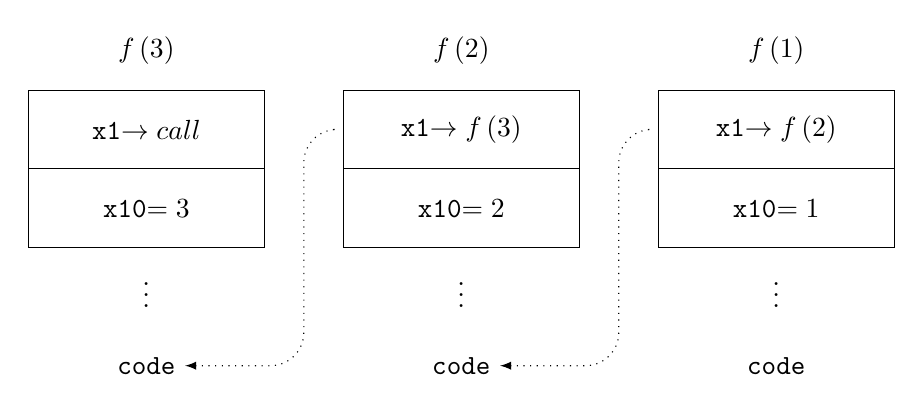
\begin{tikzpicture}
		%\draw (0,0) ++ (0,0) node(a) [draw] {$x1 \rightarrow  f\left(n\right) $};
		\draw (0,0) ++ (0,0) |-++(3,-1)|-++(-3,1);
		\draw (0,0) ++ (0,-1) ++ (0,0) |-++(3,-1)|-++(-3,1);
		\draw (0,0) ++ (1.5, -0.5) node  {\verb|x1|$ \rightarrow call$};
		\draw (0,0) ++ (1.5, -1.5) node  {\verb|x10|$ = 3 $};
		\draw (0,0) ++ (1.5, 0.5) node  {$ f\left(3\right) $};
		\draw (0,0) ++ (1.5, -2.5) node {$ \vdots $};
		\draw (0,0) ++ (1.5, -3.5) node(f3code) {\verb|code|};
		%
		\draw (4,0) ++ (0,0) |-++(3,-1)|-++(-3,1);
		\draw (4,0) ++ (0,-1) ++ (0,0) |-++(3,-1)|-++(-3,1);
		\draw (4,0) ++ (0,-0.5) node (f2x1) {};
		\draw (4,0) ++ (1.5, -0.5) node  {\verb|x1|$ \rightarrow  f\left(3\right) $};
		\draw  (4,0) ++ (1.5, -1.5) node  {\verb|x10|$ = 2 $};
		\draw (4,0) ++ (1.5, 0.5) node  {$ f\left(2\right) $};
		\draw (4,0) ++ (1.5, -2.5) node {$ \vdots $};
		\draw (4,0) ++ (1.5, -3.5) node (f2code) {\verb|code|};
		\draw [dotted, -latex, rounded corners=12pt] (f2x1)--++(-0.5,0) |- (f3code);
		%
		\draw (8,0) ++ (0,0) |-++(3,-1)|-++(-3,1);
		\draw (8,0) ++ (0,-1) ++ (0,0) |-++(3,-1)|-++(-3,1);
		\draw (8,0) ++ (0,-0.5) node (f1x1) {};
		\draw (8,0) ++ (1.5, -0.5) node  {\verb|x1|$ \rightarrow  f\left(2\right) $};
		\draw (8,0) ++ (1.5, -1.5) node  {\verb|x10|$ = 1 $};
		\draw (8,0) ++ (1.5, 0.5) node  {$ f\left(1\right) $};
		\draw (8,0) ++ (1.5, -2.5) node {$ \vdots $};
		\draw (8,0) ++ (1.5, -3.5) node (f1code) {\verb|code|};
		\draw [dotted, -latex, rounded corners=12pt] (f1x1)--++(-0.5,0) |- (f2code);
	\end{tikzpicture}
\end{center}

\subsection{Funzione foglia}
Traduciamo la seguente funzione in assembly:

\begin{lstlisting}[style=c, frame= none]
int64 esempio_foglia(int64 g, int64 h, int64 i, int64 j) { 
    int64 f;
    f = (g+h) - (i+j);
    return f;
}
\end{lstlisting}
Tale funzione è detta \underline{funzione foglia}, in quanto non chiama al suo interno nessun'altra funzione. Per questa ragione tutte le sue variabili possono evitare di essere allocate sullo stack, rendendola molto più veloce! Vediamo la traduzione, supponendo che i parametri si trovino in \verb|a0|, \verb|a1|, \verb|a2|, \verb|a3|
\begin{lstlisting}[language=assembly]
esempio_foglia:
    add a0, a0, a1  # g+h
    sub a0, a0, a2  # (g+h)-i
    sub a0, a0, a3  # ((g+h)-i)-j
    jalr x0, 0(ra)  # ritorno al chiamante
\end{lstlisting}
\subsection{Insertion sort}
\begin{lstlisting}[style = c, frame=none]
  //Funzione aux
  void sposta(int v[], size_t i) {

    size_t j;
    int appoggio = v[i];
    j = i - 1;

    while ((j >= 0) && (v[j] > appoggio)) {
      v[j+1] = v[j];
      j = j-1;
    }

    v[j+1] = appoggio;
  } 

  //Funzione sort
  void ordina(int v[], size_t n) {

    size_t i;
    i = 1;
    while (i < n) {
      sposta(v, i);
      i = i+1;
    }
  }
  \end{lstlisting}
L'algoritmo funziona scorrendo il vettore e costruendone quello ordinato inserendo di volta in volta l'\textit{i-esimo} elemento mantenendo l'ordine della porzione precedente:
Considera il seguente vettore

\begin{center}
	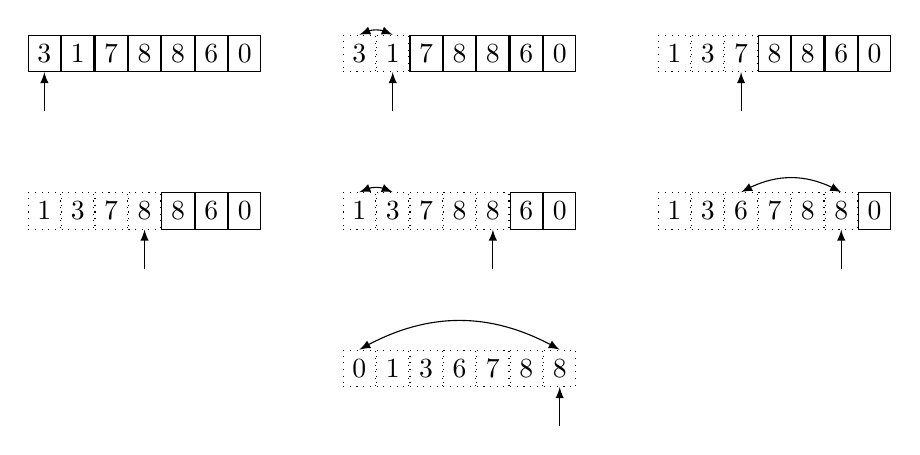
\begin{tikzpicture}
		\node (a)[draw] at (0,0) {3};
		\node (b)[draw, anchor = west] at (a.east) {1};
		\node (c)[draw, anchor = west] at (b.east) {7};
		\node (d)[draw, anchor = west] at (c.east) {8};
		\node (e)[draw, anchor = west] at (d.east) {8};
		\node (f)[draw, anchor = west] at (e.east) {6};
		\node (g)[draw, anchor = west] at (f.east) {0};
		\draw [latex-](a.south)--++(0,-0.5);
		%
		\node (a)[dotted, draw] at (4,0) {3};
		\node (b)[dotted,draw, anchor = west] at (a.east) {1};
		\node (c)[draw, anchor = west] at (b.east) {7};
		\node (d)[draw, anchor = west] at (c.east) {8};
		\node (e)[draw, anchor = west] at (d.east) {8};
		\node (f)[draw, anchor = west] at (e.east) {6};
		\node (g)[draw, anchor = west] at (f.east) {0};
		\draw [latex-](b.south)--++(0,-0.5);
		\draw [bend right, latex-latex] (b.north)to(a.north);
		%
		\node (a)[dotted, draw] at (8,0) {1};
		\node (b)[dotted,draw, anchor = west] at (a.east) {3};
		\node (c)[dotted, draw, anchor = west] at (b.east) {7};
		\node (d)[draw, anchor = west] at (c.east) {8};
		\node (e)[draw, anchor = west] at (d.east) {8};
		\node (f)[draw, anchor = west] at (e.east) {6};
		\node (g)[draw, anchor = west] at (f.east) {0};
		\draw [latex-](c.south)--++(0,-0.5);
		%
		\node (a)[dotted, draw] at (0,-2) {1};
		\node (b)[dotted,draw, anchor = west] at (a.east) {3};
		\node (c)[dotted, draw, anchor = west] at (b.east) {7};
		\node (d)[dotted, draw, anchor = west] at (c.east) {8};
		\node (e)[draw, anchor = west] at (d.east) {8};
		\node (f)[draw, anchor = west] at (e.east) {6};
		\node (g)[draw, anchor = west] at (f.east) {0};
		\draw [latex-](d.south)--++(0,-0.5);
		%
		\node (a)[dotted, draw] at (4,-2) {1};
		\node (b)[dotted,draw, anchor = west] at (a.east) {3};
		\node (c)[dotted, draw, anchor = west] at (b.east) {7};
		\node (d)[dotted, draw, anchor = west] at (c.east) {8};
		\node (e)[dotted, draw, anchor = west] at (d.east) {8};
		\node (f)[draw, anchor = west] at (e.east) {6};
		\node (g)[draw, anchor = west] at (f.east) {0};
		\draw [latex-](e.south)--++(0,-0.5);
		\draw [bend right, latex-latex] (b.north)to(a.north);
		%
		\node (a)[dotted, draw] at (8,-2) {1};
		\node (b)[dotted,draw, anchor = west] at (a.east) {3};
		\node (c)[dotted, draw, anchor = west] at (b.east) {6};
		\node (d)[dotted, draw, anchor = west] at (c.east) {7};
		\node (e)[dotted, draw, anchor = west] at (d.east) {8};
		\node (f)[dotted, draw, anchor = west] at (e.east) {8};
		\node (g)[draw, anchor = west] at (f.east) {0};
		\draw [latex-](f.south)--++(0,-0.5);
		\draw [bend right, latex-latex] (f.north)to(c.north);
		%
		\node (a)[dotted, draw] at (4,-4) {0};
		\node (b)[dotted,draw, anchor = west] at (a.east) {1};
		\node (c)[dotted, draw, anchor = west] at (b.east) {3};
		\node (d)[dotted, draw, anchor = west] at (c.east) {6};
		\node (e)[dotted, draw, anchor = west] at (d.east) {7};
		\node (f)[dotted, draw, anchor = west] at (e.east) {8};
		\node (g)[dotted, draw, anchor = west] at (f.east) {8};
		\draw [latex-](g.south)--++(0,-0.5);
		\draw [bend right, latex-latex] (g.north)to(a.north);
	\end{tikzpicture}
\end{center}


Le due funzioni, \textit{sposta} e \textit{ordina} fanno:
\begin{itemize}
	\item \textit{Sposta} prende l'elemento i-esimo e lo inserisce nel sotto vettore $ \left[0,i-1\right] $ mantenendone l'ordine
	\item \textit{Ordina} chiama la funzione \textit{sposta} per ogni suo elemento
\end{itemize}
I registri sono utilizzati nel seguente modo:
\begin{itemize}
	\item \verb|a0| = \verb|v|
	\item \verb|a1| = \verb|i| e in seguito \verb|j|
	\item \verb|a3| = \verb|appoggio|
	\item \verb|a0| = \verb|v|
	\item \verb|a0| = \verb|v|
	\item \verb|a0| = \verb|v|
\end{itemize}
\begin{lstlisting}[language = assembly]
sposta:
    slli a4,a1,2        #a4 = i*4
    add a5,a0,a4        #a5 = &v[i]
    lw a3,0(a5)         #a3 = v[i]
    addiw a1,a1,-1      #a1 = a1-1 (i-1)

    blt a1, x0, .L2     # se j < 0 esci dal ciclo
    lw a4,-4(a5)        # a4 = v[i-1]=v[j]
    bge a3,a4,.L2       # se appoggio è >= v[j] esci
    li a2,-1            # carica -1 in a2
.L3:
    sw a4,0(a5)         # memorizza v[j] (a4) in v[j+1)
    addiw a1,a1,-1      # a1 = a1-1
    beq a1,a2,.L4       # salta se a1 = -1
    addi a5,a5,-4       # j=j-1
    lw a4,-4(a5)
    bgt a4,a3,.L3       # salta se v[j] > appoggio
    j .L2
.L4:
    li a1,-1
.L2:
    addi a1,a1,1
    slli a1,a1,2
    add a1,a0,a1
    sw a3,0(a1)
    ret
 \end{lstlisting}
\section{Assembly Intel x64}
Le architetture \underline{Intel} sono nate con intenti drasticamente diversi rispetto alle architetture ARM o Risc-V. Queste architetture sono basate sui seguenti principi:
\begin{itemize}
	\item Garantire la \underline{retrocompatibilità}
	      \begin{itemize}
		      \item Eseguire codice vecchio
		      \item Lunghezza istruzioni variaible
		      \item Maggire complessità
	      \end{itemize}
\end{itemize}
Per via della sua complessità è impossibile analizzare l'intera architettura intel, ci concentreremo sulla \underline{modalità a 64 bit} (la quale garantisce retrocompatibilità con 18, 32 bit). In particolare vedremo la sintassi utilizzata dall'\underline{assemblatore GNU}
\subsection{Registri}
\begin{itemize}
	\item 16 registri
	\item Nome preceduto da \verb|%|
	\item \verb| %rax %rbx %rcx %rdx %rsx %rdx %rbp %rsp |
	\item \verb|  %r8 ... %r15|
	\item Registri specializzati:
	      \begin{itemize}
		      \item \verb| %rsp| $ \rightarrow  $ \textit{stack pointer}
		      \item \verb| %rbp| $ \rightarrow  $ \textit{base pointer}
		      \item \verb| %rip| $ \rightarrow  $ \textit{instruction pointer}
	      \end{itemize}
	\item Registri flag \verb|%rflags|: estende \verb|%eflags| che estende \verb|%flags|, ogni bit corrisponde ad una flag
	      \begin{itemize}
		      \item \verb|cf| \textit{Carry flag}
		      \item \verb|zf| \textit{Zero flag}
		      \item \verb|sign| \textit{Sign flag}
		      \item \verb|of| \textit{2's overflow flag}
	      \end{itemize}
\end{itemize}
In più i registri delle architetture intel sono divisi in sotto-registri a 32 e 16 bit come segue:
\begin{center}

	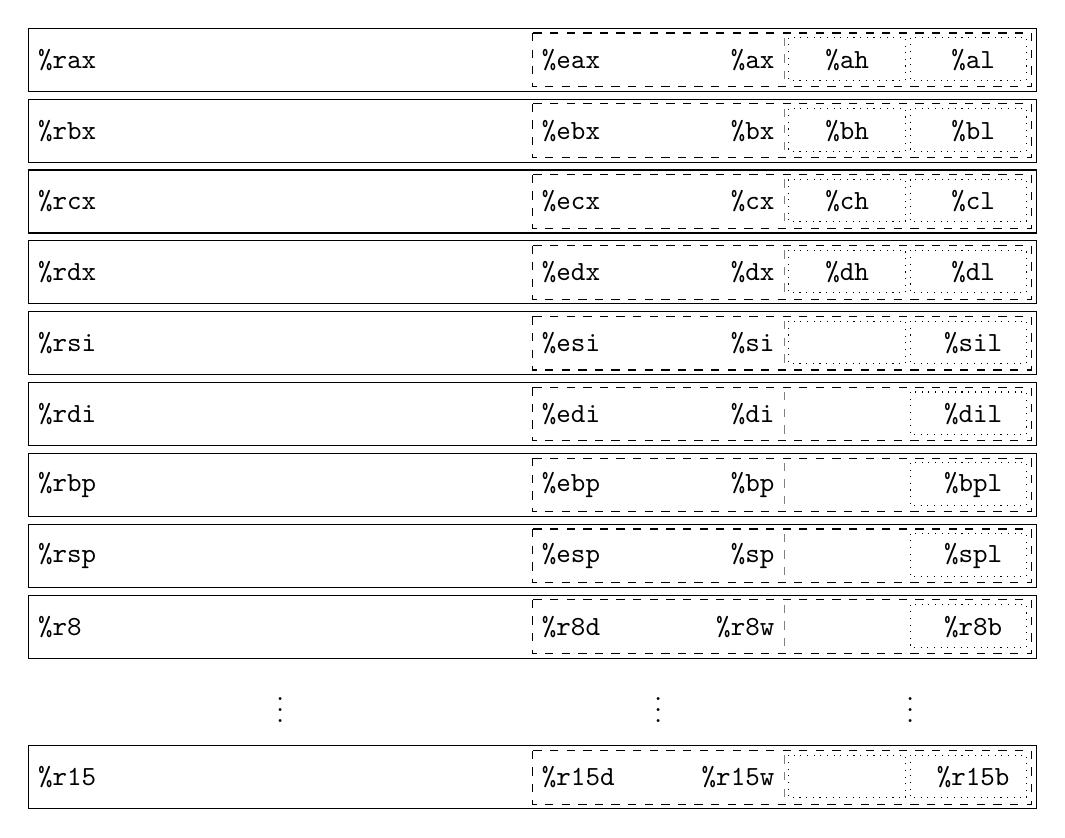
\begin{tikzpicture}[scale = 0.2]
		\foreach \x in {0,-4.5,...,-40}{
				\draw (0,\x)rectangle ++(64, -4);
			}
		\node [anchor = west] at (0,-2){\verb|%rax|
		};
		\node [anchor = west] at (0,-6.5){\verb|%rbx|
		};
		\node [anchor = west] at (0,-11){\verb|%rcx|
		};
		\node [anchor = west] at (0,-15.5){\verb|%rdx|
		};
		\node [anchor = west] at (0,-20){\verb|%rsi|
		};
		\node [anchor = west] at (0,-24.5){\verb|%rdi|
		};
		\node [anchor = west] at (0,-29){\verb|%rbp|
		};
		\node [anchor = west] at (0,-33.5){\verb|%rsp|
		};
		\node [anchor = west] at (0,-38){\verb|%r8|
		};
		%
		\foreach \x in {0,-4.5,...,-40}{
				\draw [dashed](32,\x-0.3)rectangle ++(32-0.3, -3.4);
			}
		\foreach \x in {0,-4.5,...,-40}{
				\draw [gray, dashed](48,\x -0.6) --++(0, -2.7);
			}
		\foreach \x in {0,-4.5,...,-19}{
				\draw [dotted](48.3,\x -0.6) rectangle ++(8-0.6, -2.7);
			}
		\foreach \x in {0,-4.5,...,-40}{
				\draw [dotted](56,\x -0.6) rectangle ++(8-0.6, -2.7);
			}
		%
		\node [anchor = west] at (32,-2){\verb|%eax|
		};
		\node [anchor = west] at (32,-6.5){\verb|%ebx|
		};
		\node [anchor = west] at (32,-11){\verb|%ecx|
		};
		\node [anchor = west] at (32,-15.5){\verb|%edx|
		};
		\node [anchor = west] at (32,-20){\verb|%esi|
		};
		\node [anchor = west] at (32,-24.5){\verb|%edi|
		};
		\node [anchor = west] at (32,-29){\verb|%ebp|
		};
		\node [anchor = west] at (32,-33.5){\verb|%esp|
		};
		\node [anchor = west] at (32,-38){\verb|%r8d|
		};
		%
		\node [anchor = east] at (48,-2){\verb|%ax|
		};
		\node [anchor = east] at (48,-6.5){\verb|%bx|
		};
		\node [anchor = east] at (48,-11){\verb|%cx|
		};
		\node [anchor = east] at (48,-15.5){\verb|%dx|
		};
		\node [anchor = east] at (48,-20){\verb|%si|
		};
		\node [anchor = east] at (48,-24.5){\verb|%di|
		};
		\node [anchor = east] at (48,-29){\verb|%bp|
		};
		\node [anchor = east] at (48,-33.5){\verb|%sp|
		};
		\node [anchor = east] at (48,-38){\verb|%r8w|
		};
		%
		\node  at (52,-2){\verb|%ah|
		};
		\node  at (52,-6.5){\verb|%bh|
		};
		\node  at (52,-11){\verb|%ch|
		};
		\node  at (52,-15.5){\verb|%dh|
		};
		%
		\node  at (60,-2){\verb|%al|
		};
		\node  at (60,-6.5){\verb|%bl|
		};
		\node  at (60,-11){\verb|%cl|
		};
		\node  at (60,-15.5){\verb|%dl|
		};
		\node  at (60,-20){\verb|%sil|
		};
		\node  at (60,-24.5){\verb|%dil|
		};
		\node  at (60,-29){\verb|%bpl|
		};
		\node  at (60,-33.5){\verb|%spl|
		};
		\node  at (60,-38){\verb|%r8b|
		};
		\node (a) [anchor = north, outer sep = 5pt] at (16, - 40) {$ \vdots $};
		\node [anchor = north, outer sep = 5pt]at (40, - 40) {$ \vdots $};
		\node [anchor = north, outer sep = 5pt]at (56, - 40) {$ \vdots $};

		\draw (a.south -| 0,0) rectangle ++(64, -4);
		\draw [dashed](a.south -| 0,0)++(32,-0.3)rectangle ++(32-0.3, -3.4);
		\draw [gray, dashed](a.south -| 0,0)++(48, -0.6) --++(0, -2.7);
		\draw [dotted](a.south -| 0,0)++ (48.3, -0.6) rectangle ++(8-0.6, -2.7);
		\draw [dotted](a.south -| 0,0) ++(56, -0.6) rectangle ++(8-0.6, -2.7);
		\draw (a.south -| 0,0)++(0,-2) node [anchor = west] {\verb|%r15|
		};
		\draw (a.south -| 0,0)++(32,-2) node [anchor = west] {\verb|%r15d|
		};
		\draw (a.south -| 0,0)++(48,-2) node [anchor = east] {\verb|%r15w|
		};
		\draw (a.south -| 0,0)++(60,-2) node  {\verb|%r15b|
		};
	\end{tikzpicture}
\end{center}
\subsubsection*{Convenzioni di chiamata}
Ricordiamo che queste non fanno parte dell'ISA ma dell'\underline{ABI}
\begin{itemize}
	\item Primi 6 argomenti in \verb| %rdi %rsi %rdx %rcx %r8 %r9|
	\item Valori di ritorno in \verb|%rax %rdx|
\end{itemize}
\begin{table}[H]
	\begin{center}
		\begin{tabular}{|l|l|l|}
			\hline
			Register    & Description                         & Saver                   \\
			\hline
			\verb|%rax| & Return value                        & Caller                  \\
			\verb|%rbx| & Saved register                      & Callee                  \\
			\hline
			\verb|%rcx| & \multirow{4}{*}{Function arguments} & \multirow{4}{*}{Caller} \\
			\verb|%rdx| &                                     &                         \\
			\verb|%rsi| &                                     &                         \\
			\verb|%rdi| &                                     &                         \\
			\hline
			\verb|%rbp| & Base pointer                        & \multirow{2}{*}{Caller} \\
			\verb|%rsp| & Stack pointer                       &                         \\
			\hline
			\verb|%r8|  & \multirow{2}{*}{Function arguments} & \multirow{2}{*}{Caller} \\
			\verb|%r9|  &                                     &                         \\
			\hline
			\verb|%r10| & \multirow{2}{*}{Temporaries}        & \multirow{2}{*}{Caller} \\
			\verb|%r11| &                                     &                         \\
			\hline
			\verb|%r12| & \multirow{4}{*}{Saved registers}    & \multirow{4}{*}{Callee} \\
			\verb|%r13| &                                     &                         \\
			\verb|%r14| &                                     &                         \\
			\verb|%r15| &                                     &                         \\
			\hline
		\end{tabular}
	\end{center}
	\caption{Uso dei registri in Intel x64}
\end{table}
\subsubsection*{Struttura istruzioni}
Tutti i registri sono preceduti da \verb|%|, mentre gli immediati da \verb|$|
\begin{itemize}
	\item Tendenzialmente hanno due operandi
	      \begin{itemize}
		      \item Primo operando \textit{sorgente}
		      \item Secondo operando \textit{destinazione implicita}
	      \end{itemize}
\end{itemize}
\textbox{Destinazione e sorgente possono essere registri, memoria o immediati. Tuttavia vige la limitazione che non possono essere entrambi \underline{indirizzi di memoria}}
\subsubsection*{Modalità di indirizzamento}
Sono molto più complesse rispetto al Risc-V. Hanno la seguente forma:
\begin{center}
	\verb|<displacement> (<base reg>, <index reg>, <scale>)|
\end{center}
\begin{itemize}
	\item \textit{Valore immediato} in byte, di quanto va shiftato l'indirizzo (come Risc-V)
	\item Registro contenente l'indirizzo di memoria a cui accedere
	\item Indice si usa solo se si indica anche scala e viceversa. Shiftano l'indirizzo di \verb|<index reg> * <scale>|
\end{itemize}
\section{Assembly ARM}
\begin{itemize}
	\item 16 registri quasi tutti registri \underline{generl purpuse} numerati da \verb|r0 ... r15| con nome simbolito (ad esempio \verb|r13 = sp| o \verb|r14 = lr|, ossia \textit{stack pointer e link register})
	\item Utilizza flags per istruzioni condizionali
	\item \underline{Ogni} istruzione può essere resa condizionale, postponendo determinate sillabe
	\item Gli immediati vengono indicati con \verb|#|
\end{itemize}
\begin{table}[H]
	\begin{center}
		\begin{tabular}{|l|l|l|}
			\hline
			Register      & Description                          & Saver                   \\
			\hline
			\verb|r0|     & \multirow{2}{*}{Return values}       & \multirow{4}{*}{Caller} \\
			\verb|r1|     &                                      &                         \\
			\cline{2-2}
			\verb|r2|     & \multirow{2}{*}{Function parameters} &                         \\
			\verb|r3|     &                                      &                         \\
			\hline
			\verb|r4-r11| & Saved registers                      & Callee                  \\
			\hline
			\verb|r12|    & Temporary register                   & Caller                  \\
			\verb|r13|    & Stack pointer                        & Callee                  \\
			\verb|r14|    & Return address                       & Callee                  \\
			\verb|r15|    & Program counter/flags                & /                       \\
			\hline
		\end{tabular}
	\end{center}
	\caption{Uso dei registri in ARM}
\end{table}
I flag sono contenuti nei bit più significativi del registro \verb|r15| in una sotto porzione chiamata \verb|apsr|. Questi sono:
\begin{itemize}
	\item \verb|z| se è 0
	\item \verb|n| se è negativo
	\item \verb|c| se è avvenuto un overflow fra dati unsigned
	\item \verb|v| se è avvenuto un overflow fra dati signed
\end{itemize}
\textbox{In ARM \underline{tutte} le istruzioni possono essere rese condizionali postponendo le seguenti sillabe dopo l'istruzione}
Tramite questi bit possiamo veribicare le seguenti condizioni:
\begin{itemize}
	\item \verb|eq| \textit{equal}
	\item \verb|ne| \textit{not equal}
	\item \verb|hs| \textit{higher or same}
	\item \verb|lo| \textit{lower}
	\item \verb|mi| \textit{minus}
	\item \verb|pl| \textit{plus}
	\item \verb|vs| \textit{overflow}
	\item \verb|vc| \textit{overflow clear}
	\item \verb|hi| \textit{higher}
	\item \verb|ls| \textit{lower or same}
	\item \verb|ge| \textit{greater or equal}
	\item \verb|it| \textit{less than}
	\item \verb|gt| \textit{greater than}
	\item \verb|le| \textit{less or equal}
\end{itemize}
\subsection{Modalità di indirizzamento}
La sintatti per indicare un indice è della forma seguente:
\begin{center}
	\verb|i = <base> + {<offset>  <indice (shiftato)>}|
\end{center}
\subsubsection*{Pre e post indexing}
In ARM, il valore del registro di base può essere aggiornato direttamente nell'istruzione di indirizzamento.
\begin{itemize}
	\item \textit{Pre-indexing}:
	      \begin{itemize}
		      \item Senza writeback: Accedo all'indirizzo e lascio \verb|<base>| invariato
		      \item  Con writeback: salvo indirizzo calcolato in \verb|<base>|
	      \end{itemize}
	\item \textit{Post-indexing}:
	      \begin{itemize}
		      \item Solo con writeback: accedo all'idirizzo indicato in \verb|<base>| e ci accedo. Poi aggiorno base con il valore indicato
	      \end{itemize}
\end{itemize}
Ad esempio:
\begin{itemize}
	\item Pre index - \underline{no} writeback : \verb|ld r0, [r1, #4]| $ \rightarrow  $ \verb|r0 = [r1 + 4]|, \verb|r1| invariato
	\item Pre index - writeback: \verb|ld r0, [r1, #4]!| $ \rightarrow  $ \verb|r0 = mem[r1+4]|, \verb|r1 = r1 + 4|
	\item Post index - writeback: \verb|ld r0, [r1], #4| $ \rightarrow  $ \verb|r0 = mem[r1]|, \verb|r1 = r1 + 4|
\end{itemize}
Inoltre posso usare indice shiftato come segue
\begin{center}
	\verb|ldr r0, [r1, r2, lsl #4]| ossia \verb|r0 = mem[r1 + r2 << 4]|
\end{center}
\subsection{Letture e scritture multiple}

\section{Toolchain}
Abbiamo visto che un processore è in grado di "leggere" sequenze di bit, chiamate instruzioni. Tuttavia per noi è troppo complicato andare a scrivere un programma avanzato in Assembly (il quale costituisce un insieme di codici mnemonici tramite i quali vengono convertiti direttamente in stringe binarie). Per questa ragione il codice assembly viene generato a partire da un linguaggio ad alto livello, ad esempio \verb|c| o \verb|c++|
\textbox{Una toolchain fornisce gli strumenti adeguati al fine di poter passare da un linguaggio di alto livello a linguaggio macchina}:
\begin{center}
	\begin{tikzpicture}
		\node (a)[draw] at (0,0) {Programma c};
		\draw (a.south) --++ (0,-0.5) node (b)[draw, ellipse, anchor = north]  {Compilatore};
		\draw (b.south) --++ (0,-0.5) node (c)[draw, anchor = north]  {Programma in linguaggio assembler};
		\draw (c.south) --++ (0,-0.5) node (d)[draw, ellipse, anchor = north]  {Assembler};

		\draw (d.south)   ++ (0,-0.5) node (e)[draw, , anchor = north]  {Oggetto: modulo in linguaggio macchina};
		\draw (e.south)   ++ (0,-0.5) node (f)[draw, , anchor = north]  {Oggetto: funzioni di libreria (linguaggio macchina)};

		\draw (f.south) ++ (0,-0.5) node (g)[draw, ellipse, anchor = north]  {Linker};
		\node (fit)[fit= (e) (f), draw, dashed] {};
		\draw (d)--(fit.north);
		\draw (fit.south)--(g);
		\draw (g.south) --++ (0,-0.5) node (h)[draw, anchor = north]  {Eseguibile: programma in linguaggio macchina};
		\draw (h.south) --++ (0,-0.5) node (h)[draw, ellipse, anchor = north]  {Loader};
		\draw (h.south) --++ (0,-0.5) node (h)[draw,  anchor = north]  {Memoria};
	\end{tikzpicture}
\end{center}
Possiamo, ad esempio attraverso il \textit{gnu compiler collection} o \verb|gcc|, far si che il processo di compilazione si fermi prima, tramite i seguenti comandi:
\command{gcc }{-S}{}{ferma la compilazione dopo aver generato il file assembly}
\command{gcc }{-c}{}{ferma la compilazione dopo aver generato il file oggetto}
Nota che il gcc è formato da 4 sottoprogrammi:
\begin{itemize}
	\item \verb|cpp| è il preprocessor, risolve le macro e gli import
	\item \verb|cc| traduce il programma in codice assembly
	\item \verb|as| assemblatore, traduce l'assembly in linguaggio macchina
	\item \verb|ld| esegue il linking, ossia aggiunge le librerie
\end{itemize}
\subsubsection*{Assemblatore}
L'assemblatore spesso fa più che tradurre con corrispondenza diretta le istruzioni assembly in istruzioni macchina, ad esempio:
\begin{itemize}
	\item Converte pseudo istruizioni
	      \begin{itemize}
		      \item \verb|j LABEL| diventa \verb|jal x0, LABEL|
		      \item \verb|mv x10, x11| diventa \verb|addi x10, x11, 0|
	      \end{itemize}
	\item Converte numeri da esadecimale/decimale a binario
	\item Converte le label in indirizzi di memoria contenenti l'istruzione
	\item Gestrisce salti troppo ampi (nell'istruzione jump abbiamo un numero limitato di byte per indicare lo spiazzamento)
	\item Genera metadati
\end{itemize}
\subsubsection*{File oggetto}
I file oggetto sono i file che verranno poi linkati. Contengono le seguenti informazioni, divise in \underline{segmenti}:
\begin{itemize}
	\item \textit{Header}: specifica la dimensione e la posizione degli altri segmenti
	\item \textit{Segmenti}
	      \begin{itemize}
		      \item \textit{Segmento di testo}: contiene il codice in linguaggio macchina
		      \item \textit{Segmento di dati}: contiene tutti i dati allocati durante la durata del programma
	      \end{itemize}
	\item \textit{Tabella dei simboli}:
	      \begin{itemize}
		      \item Associa i simboli (varibili, funzioni) ad indirizzi relativi
		      \item Enumera simboli non definiti (sono definiti altrove)
	      \end{itemize}
	\item \textit{Tabella di rilocazione}
	      \begin{itemize}
		      \item Se, ad esempio, una jump punta ad un'indirizzo assoluto e non relativo all'indirizzo dell'istruzione corrente, questo va a finire nella suddetta tabella, in quando deve essere patchato
	      \end{itemize}
\end{itemize}
Il linker si occupa quindi principalmente di mettere in ordine e concatenare opportunamente questi file oggetto, eliminando dunque le symbol e relocation tables
\subsubsection*{Librerie}
Una libreria non è altro che una collezione di file oggetto. Ne esistono di due tipi:
\begin{itemize}
	\item \textit{Statiche} con estensione \verb|.a|. Linkate da \verb|ld|
	      \begin{itemize}
		      \item Migliore velocità di esecuzione
		      \item Maggiore peso del programma
		      \item Programma autocontenuto in un solo eseguibile
		      \item Più semplici
	      \end{itemize}
	\item \textit{Dinamiche} con estensione \verb|.so|. Linkate a \underline{runtime}
	      \begin{itemize}
		      \item Meno efficienti
		      \item Programma più leggero in termini di byte
		      \item Programma le necessita a runtime (eseguibile non autoconenuto)
		      \item Più complicate da implementare
	      \end{itemize}
\end{itemize}
Inoltre con le librerie dinamiche, è possibile anche seguire il cosiddetto lazy loading:
\begin{itemize}
	\item Solitamente le librerie vengono caricate dal \textit{sistema operativo} all'avvio del programma
	\item Per ridurre questi tempi è possibile rimandare il caricamento al momento in cui una libreria viene utilizzata
	\item Quando si chiama una funzione di libreria per la prima volta, viene chiamato uno \underline{stub}, che esegue il suo caricamento durante runtime
	\item La \underline{seconda volta} che la funzione viene chiamata, questa sarà gia linkata e quindi verrà \underline{usata direttamente}
\end{itemize}
\section{Il processore}
Affrontiamo ora come funziona un processore, facendo riferimento all'ISA Risc-V.
\subsubsection*{Primi passi esecuzioe}
Nell'esecuzione delle istruzioni, sono sempre presenti due passi:
\begin{itemize}
	\item \textit{Fetch} ossia  il prelievo dell'istruzione:
	      \begin{itemize}
		      \item Vado a indirizzo puntato da \textit{program counter}
		      \item Leggo contenuto (32 bit nel caso Risc-V)
	      \end{itemize}
	\item \textit{Lettura registri}. Vengono letti i registri coinvolti nell'istruzione
\end{itemize}
ciò che avviene dopo dipende da architettura a architettura
\subsubsection*{ALU}
Tutti i tipi di istruzioni utilizzano la \textit{alu} (Unità Logico Aritmetica).
Tutte le istruzioni la utilizzano:
\begin{itemize}
	\item \textit{Accessi a memoria} (calcolo indirizzo)
	\item \textit{Istruzioni aritmetico/ logiche}
	\item \textit{Salti condizionati} (per verificare se sono uguali due registri)
\end{itemize}
%\begin{circuitikz}
%	%
%	\draw (0,0) |-++ (1,1.5) |-++(-1, -3) -- cycle;
%	\draw (2,0) |-++ (4,2) |-++(-4, -4) -- cycle;
%	\node (indirizzo)[anchor = west] at (2,0) {Indirizzo};
%	\node (istruzione)[anchor = east] at (6,0) {Istruzione};
%	\node (memoria istruzioni)[anchor = south] at (4,-2) {\textit{Memoria istruzioni}};
%	\node at (0.5,0) {PC};
%	\draw [-latex](1,0)--(indirizzo.west);
%	%
%	\draw (7,0) |-++ (4,2) |-++(-4, -4) -- cycle;
%	\node (dato)[anchor = west] at (7,1.5) {Dato};
%	\node (registro1)[anchor = west] at (7,0.5) {Registro 1};
%	\node (registro2)[anchor = west] at (7,-0.5) {Registro 2};
%	\node (registron)[anchor = west] at (7,-1.5) {Registro $ \ldots  $};
%	\node (registri)[anchor = east] at (11,0) {\textit{Registri}};
%	\node (aludx)[ALU, anchor= west] at (12, 0){\rotatebox {90}{\small \ttfamily ALU}};
%	%
%	\draw (aludx)++ (0, 3) -|++ (-1.5,4) -|++(3, -4) -- cycle;
%	\draw (aludx)++ (0, 3) ++ (-1.5, 2)++ (0, -1.5) node[anchor = west]{Dato};
%	\draw (aludx)++ (0, 3) ++ (-1.5, 2)++ (0, 1.5) node[anchor = west]{Indirizzo};
%	\draw (aludx)++ (0, 3) ++ (-1.5, 2)++ (3, 0) node[anchor = east]{Memoria dati};
%	%\node [ALU] {\rotatebox {90}{\small \ttfamily ALU}};
%	\draw [-latex] (istruzione.east) --++(0.5, 0) node [blackdot]{}|- (registro1)node[blackdot, midway]{};
%	\draw [-latex] (istruzione.east) --++(0.5, 0) |- (registro2) node[blackdot, midway]{};
%	\draw [-latex] (istruzione.east) --++(0.5, 0) |- (registron) node[blackdot, midway]{};
%	\draw [latex-](aludx.blpin 1)--++(-1, 0);
%	\draw [latex-](aludx.blpin 2)--++(-1, 0);
%\end{circuitikz}
\begin{figure}[H]
	\begin{center}
		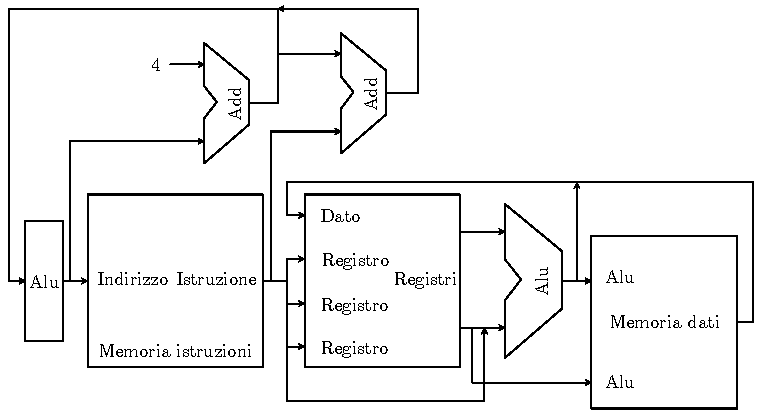
\includegraphics{Images/Datapath1.pdf}
	\end{center}
	\caption{Datapath 1}
\end{figure}
Tuttavia, questa prima immagine risulta molto approssimativa, in quanto è necessario \underline{coordinare tramite dei mux} quale dato sceglere laddove si presentino diramazioni. Ciò è fatto grazie ai nuovi elementi introdotti in tratteggiato:
\begin{figure}[H]
	\begin{center}
		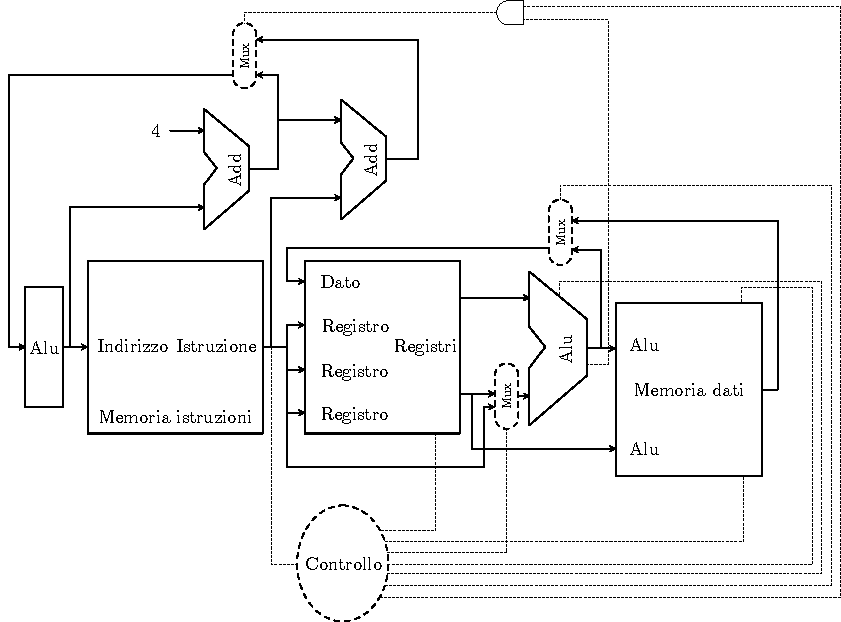
\includegraphics{Images/Datapath2.pdf}
	\end{center}
	\caption{Datapath 2, con aggiunta di elementi di controllo}
\end{figure}
Nota che quasi tutti i segnali in uscita sono a 1 bit, ad eccezione del segnale che entra all'interno dell'ALU. Quel messagio codifica l'operazione che deve eseguire la alu
\section{Memoria}
\subsection{La cache}
\textbox{Nella creazione di dispositivi capaci di immagazzinare dati, c'è sempre un trade off fra efficienza nell'accesso e dimensione dell'archivio. Per questo si usano diverse \underline{gerarchie di memoria}, per ottenere il compromesso ideale}
Immagina di avere immagazzinato dei dati un un archivio. Ogni volta che devo estrarre un dato devo alzarmi dalla scrivania e prendere il fascicolo corrispondente. Il 90\% di tempo verrà utilizzato proprio per andare dalla scrivania all'archivio. In alternativa posso portare tutti tutti i fascicoli sulla scrivania risparmiando tempo. Le gerarchie di memoria sono le seguenti:
\begin{itemize}
	\item \textit{Registri} - velocissimi ma capacità ridottissima
	\item \textit{Cache} - intermedio fra memoria principale e registri
	\item \textit{Memoria principale} - lenta ma molto capiente
\end{itemize}
\begin{tabular}{|l|l|l|l|}
	\hline Tecnologia & Tempo di accesso tipico         & $\$$ per GB (2010) & \$ per GB (2012) \\
	\hline
	SRAM              & $0.5-2.5 \mathrm{~ns}$          & $\$ 2000-\$ 5000$  & $\$ 500-\$ 1000$ \\
	DRAM              & $50-70 \mathrm{~ns}$            & $\$ 20-\$ 75$      & $\$ 10-\$ 20$    \\
	Memoria flash     & $70-150 \mathrm{~ns}$           & $\$ 4-\$ 12$       & $\$ 0.75-\$ 1$   \\
	Dischi magnetici  & $5000000-20000000 \mathrm{~ns}$ & $\$ 0.2-\$ 2$      & $\$ 0.05-\$ 0.1$ \\
	\hline
\end{tabular}
\subsubsection*{Struttura gerarchia della memoria}
La memoria, per le ragioni elencate prima, è strutturata ponendo:
\begin{itemize}
	\item Memoria a bassa capacità e alta velocità \textit{vicino} al processore
	\item Memoria ad alta capacità e bassa velocità \textit{lontano} al processore
\end{itemize}
Per questa ragione è necessario implementare meccanismi che controllino a quale livello della gerarchia è disponibile un determinato dato
\subsubsection*{Terminologia}
\begin{itemize}
	\item \underline{Blocco} unità minima di informazione che può essere presente o assente in ciascun livello
	\item \underline{Hit rate} frequenza con cui trovo il dato nel livello superiore
	\item \underline{Miss rate} complementare dell'hit rate: $ \rightarrow  $ 1 - hit rate
	\item \underline{Tempo di hit} quanto tempo serve per accedere ad un dato se è presente al livello corrente
	\item \underline{Penalità di miss} quanto tempo devo sprecare per accedere al dato se devo andare al livello più distante dal processore
\end{itemize}
\textbox{Il tempo di hit è di molto maggiore rispetto alla penalità di miss, per questa ragione è vantaggioso implementare gerarchie di memoria}
\subsection{Tipo di cache}
\subsubsection*{Cache a mappatura diretta}
Come posso verificare se un dato è presente o meno in cache? Questo meccanismo di mappatura è implementato diversamente in diversti tipi di cache
\begin{itemize}
	\item \textit{Cache a mappatura diretta}. Ogni indirizzo della memoria principale è mappato ad un indirizzo della memoria cache tramite il modulo:
	      \[
		      \text{ Indirizzo cache } = \text{ indirizzo principale } \%  \text{ dimensione cache }
	      \]
\end{itemize}
\subsubsection*{Gestione delle miss}
Nel momento in cui \underline{non} abbiamo miss, la presenza della cache non altera di molto il funzionamento di un processore. Se c'è una miss, tuttavia, dovra succedere una cosa del tipo:
\begin{itemize}
	\item Inviare il valore \textit{program counter} - 4 alla memoria (incremento viene eseguito all'inizio)
	\item Comandare la memoria di eseguire una lettura e attenderne il completamento
	\item Scrivere il blocco che proviene dalla memoria della cache aggiornando il tag
	\item Far ripartire l'istruzione dal fetch, che stavolta troverà l'istruzione in cache
\end{itemize}
\subsubsection*{Tag}
Il tag è una parte di memoria cache che serve ad indicare quale indirizzo di memoria è salvato all'interno di un determinato blocco di cache
\vskip3mm
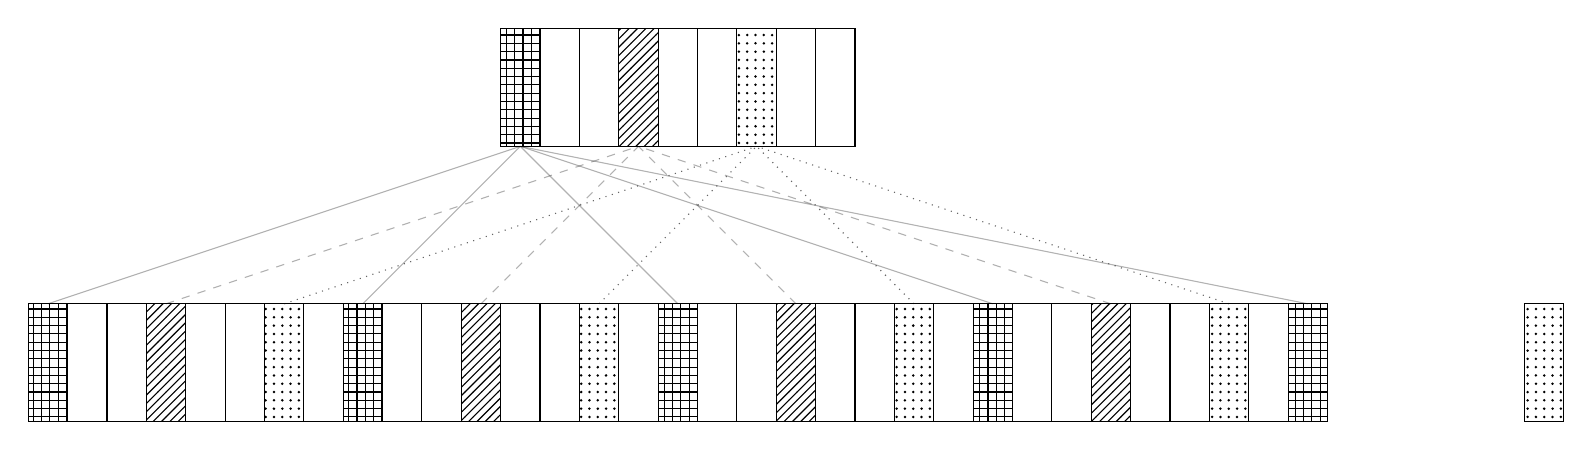
\begin{tikzpicture}[scale = 0.5]
	\foreach\x in {0,...,8}{
			\draw (\x,0) rectangle ++(1,-3);
		}
	\foreach\x in {0,...,32}{
			\draw (\x-12,-7) rectangle ++(1,-3);
		}
	\foreach\x in {0,8,...,32}{
			\draw [pattern = dots](\x-6,-7) rectangle ++(1,-3);
		}
	\foreach\x in {0,8,...,30}{
			\draw [pattern = north east lines](\x-9,-7) rectangle ++(1,-3);
		}
	\foreach\x in {0,8,...,32}{
			\draw [pattern = grid](\x-12,-7) rectangle ++(1,-3);
		}

	\foreach \x in {0,8,...,32}{
			\draw [opacity = 0.3](-11.5+\x,-7)--(0.5,-3);
		}
	\foreach \x in {0,8,...,30}{
			\draw [dashed, opacity = 0.3](-8.5+\x,-7)--(3.5,-3);
		}
	\foreach \x in {0,8,...,30}{
			\draw [dotted, opacity = 0.6](-5.5+\x,-7)--(6.5,-3);
		}
	\draw [pattern = grid](0,0) rectangle ++(1,-3);
	\draw [pattern = north east lines](3,0) rectangle ++(1,-3);
	\draw [pattern = dots](6,0) rectangle ++(1,-3);
\end{tikzpicture}
\vskip3mm
Ad esempio prendiamo il primo blocco di cache a sinistra: in questo caso tutti il tag ci dirà quale dei blocchi corrispondendi nella memoria principale corrispondono a quest'ultimo. In particolare supponiamo di avere:
\begin{itemize}
	\item Indirizzo su 64 bit
	\item Dimensione della cache $ = 2^{n} $
	\item Dimensione del blocco di cache $ = 2 ^{m} $ words = $ 2^{m+2} $ bytes
\end{itemize}
allora:
\[
	\text{ dimensione tag } = 64 - n - m - 2
\]
\subsubsection*{Cache completamente associativa}
Dato un indirizzo di memoria, anzichè avere una mappatura 1:1 con la sua posizione nella cache, devo cercare all'interno di \underline{tutta} la cache e verificare se è presente il dato che ricerco.
\begin{itemize}
	\item Vantaggi:
	      \begin{itemize}
		      \item Ogni dato può essere salvato ovunque nella cache. Se in una cache \underline{a mappatura diretta} ho bisogno di un dato che si mappa nella stessa zona della cache spesso, allora avrà molti miss. Questo problema non si presenta con la cache associativa
	      \end{itemize}
	\item Svantaggi:
	      \begin{itemize}
		      \item Costosissima da realizzare
		      \item Il tag è sempre l'intero indirizzo di memoria
		      \item Ho bisongo di $ n $ comparatori per ricercare efficacemente l'indirizzo all'interno della cache
	      \end{itemize}
\end{itemize}
\subsubsection*{Cache set-associativa}
Posso mischiare le tecnologie di cache a mappatura diretta ed associativa per ottenere la \underline{cache set-associativa}. In particolare in questa cache avrò che
\begin{itemize}
	\item Un indirizzo in memoria è mappato ad un insieme di blocchi detto \underline{linea} \textit{cache a mappatura diretta}
	\item All'interno della linea, la ricerca del blocco avviene tramire $ n $ comparatori \textit{cache puramente associativa}
\end{itemize}
\begin{figure}[H]
	\begin{subfigure}{0.5\textwidth}
		\begin{center}
			\begin{tabular}{ccccc}
				Linea                  & Tag                   & Dato                  & Tag                   & Dato                  \\ \cline{2-5}
				\multicolumn{1}{c|}{0} & \multicolumn{1}{c|}{} & \multicolumn{1}{c|}{} & \multicolumn{1}{c|}{} & \multicolumn{1}{c|}{} \\ \cline{2-5}
				\multicolumn{1}{c|}{1} & \multicolumn{1}{c|}{} & \multicolumn{1}{c|}{} & \multicolumn{1}{c|}{} & \multicolumn{1}{c|}{} \\ \cline{2-5}
				\multicolumn{1}{c|}{2} & \multicolumn{1}{c|}{} & \multicolumn{1}{c|}{} & \multicolumn{1}{c|}{} & \multicolumn{1}{c|}{} \\ \cline{2-5}
				\multicolumn{1}{c|}{3} & \multicolumn{1}{c|}{} & \multicolumn{1}{c|}{} & \multicolumn{1}{c|}{} & \multicolumn{1}{c|}{} \\ \cline{2-5}
			\end{tabular}
		\end{center}
		\caption{Set associative cache a 2 vie}
	\end{subfigure}
	%
	\begin{subfigure}{0.5\textwidth}
		\begin{center}
			\begin{tabular}{ccc}
				Linea                  & Tag                   & Dato                  \\ \cline{2-3}
				\multicolumn{1}{c|}{0} & \multicolumn{1}{c|}{} & \multicolumn{1}{c|}{} \\ \cline{2-3}
				\multicolumn{1}{c|}{1} & \multicolumn{1}{c|}{} & \multicolumn{1}{c|}{} \\ \cline{2-3}
				\multicolumn{1}{c|}{2} & \multicolumn{1}{c|}{} & \multicolumn{1}{c|}{} \\ \cline{2-3}
				\multicolumn{1}{c|}{3} & \multicolumn{1}{c|}{} & \multicolumn{1}{c|}{} \\ \cline{2-3}
				\multicolumn{1}{c|}{4} & \multicolumn{1}{c|}{} & \multicolumn{1}{c|}{} \\ \cline{2-3}
				\multicolumn{1}{c|}{5} & \multicolumn{1}{c|}{} & \multicolumn{1}{c|}{} \\ \cline{2-3}
				\multicolumn{1}{c|}{6} & \multicolumn{1}{c|}{} & \multicolumn{1}{c|}{} \\ \cline{2-3}
				\multicolumn{1}{c|}{7} & \multicolumn{1}{c|}{} & \multicolumn{1}{c|}{} \\ \cline{2-3}
			\end{tabular}
		\end{center}
		\caption{Set associative cache a 1 via (\textit{a mappatura diretta})}
	\end{subfigure}
	%
	\vskip10mm
	\begin{subfigure}{\textwidth}
		\begin{center}
			\begin{tabular}{ccccccccc}
				Linea                  & Tag                   & Dato                  & Tag                   & Dato                  & Tag                   & Dato                  & Tag                   & Dato                  \\ \cline{2-9}
				\multicolumn{1}{c|}{0} & \multicolumn{1}{c|}{} & \multicolumn{1}{c|}{} & \multicolumn{1}{c|}{} & \multicolumn{1}{c|}{} & \multicolumn{1}{c|}{} & \multicolumn{1}{c|}{} & \multicolumn{1}{c|}{} & \multicolumn{1}{c|}{} \\ \cline{2-9}
				\multicolumn{1}{c|}{1} & \multicolumn{1}{l|}{} & \multicolumn{1}{l|}{} & \multicolumn{1}{l|}{} & \multicolumn{1}{l|}{} & \multicolumn{1}{l|}{} & \multicolumn{1}{l|}{} & \multicolumn{1}{l|}{} & \multicolumn{1}{l|}{} \\ \cline{2-9}
			\end{tabular}
		\end{center}
		\caption{Set associative cache a 4 vie}
	\end{subfigure}
	\vskip10mm
	\begin{subfigure}{\textwidth}
		\begin{center}
			\begin{tabular}{ccccccccccccc}
				Linea                  & Tag                   & Dato                  & Tag                   & Dato                  & Tag                   & Dato                  & Tag                   & Dato                  & Tag                   & Dato                  & Tag                   & Dato                  \\ \cline{2-13}
				\multicolumn{1}{c|}{0} & \multicolumn{1}{c|}{} & \multicolumn{1}{c|}{} & \multicolumn{1}{c|}{} & \multicolumn{1}{c|}{} & \multicolumn{1}{c|}{} & \multicolumn{1}{c|}{} & \multicolumn{1}{c|}{} & \multicolumn{1}{c|}{} & \multicolumn{1}{c|}{} & \multicolumn{1}{c|}{} & \multicolumn{1}{c|}{} & \multicolumn{1}{c|}{} \\ \cline{2-13}
			\end{tabular}
		\end{center}
		\caption{Set associative cache a 8 vie (\textit{completamente associativa})}
	\end{subfigure}
	\caption{Configurazioni diverse di cache}
\end{figure}
\begin{figure}[H]
	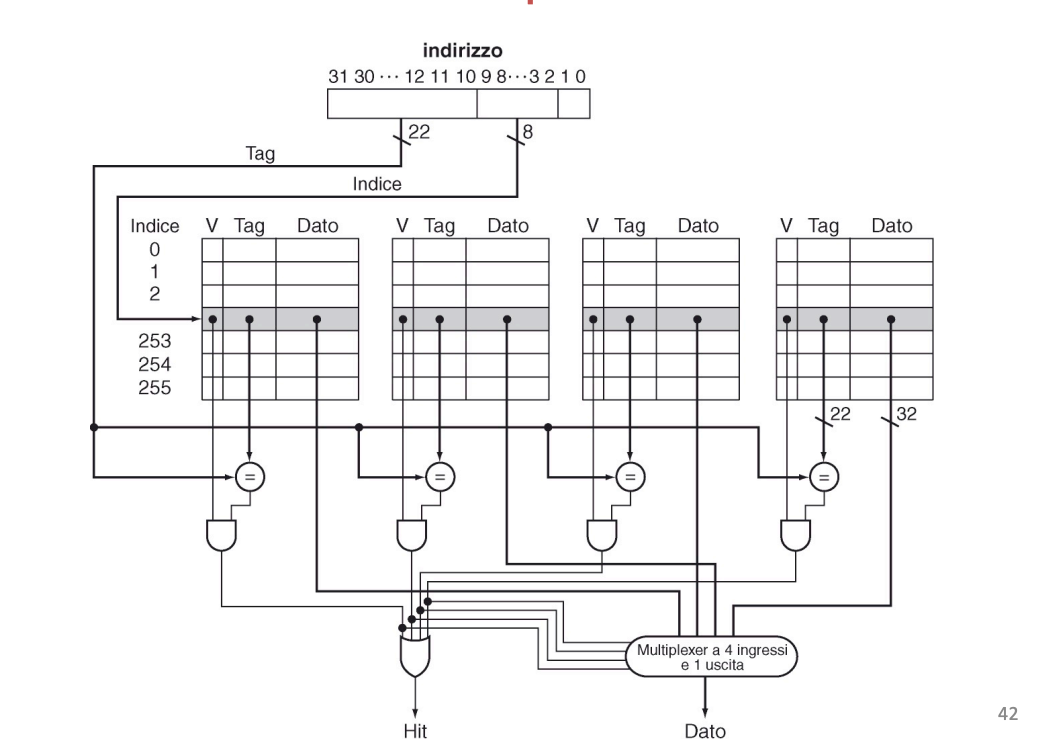
\includegraphics[width = \textwidth]{Images/cache a 4 vide.png }
	\caption{Esempio implementazione cache a 4 vie}
\end{figure}
\textbox{Nota che nella cache a mappatura diretta se avviene un miss poi nella cache so in quale indirizzo caricare il nuovo dato. Ciò \underline{non è vero} per una cache associativa}
Esistono più policy per risolvere questo problema:
\begin{itemize}
	\item Policy \underline{FIFO}
	\item Policy \underline{Least Recently Used} (usa una sequenza di bit per memorizzare l'ultimo accesso)
\end{itemize}
\section{Input-output}
Un calcolatore sarebbe inutile se non ci fosse un modo per interfacciavisi. Ciò viene reso possibile da dispositivi \textit{input-output}. I dispositivi sono collegati al processore tramite un \textit{dispositivo di comunicazione} chiamato \underline{bus}:
\begin{figure}[H]
	\begin{center}
		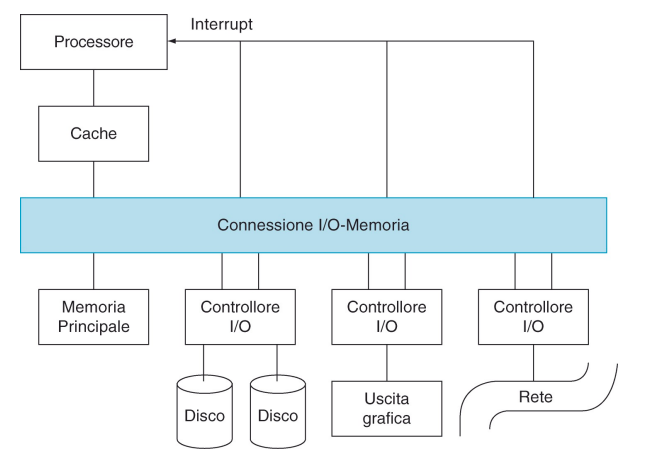
\includegraphics[width = 0.7\textwidth]{Images/bus.png }
	\end{center}
	\caption{Esempio semplicifato del bus}
\end{figure}
\subsubsection*{Caratterizzazione}
I dispositivi io sono caratterizzati da:
\begin{itemize}
	\item \textit{Comportamento}: possono effettuare operazioni di lettura o scrittura (R/W)
	\item \textit{Partner}: può essere uomo o macchina
	\item \textit{Velocità di trasferimento}
\end{itemize}
\begin{center}
	\begin{tabular}{|c|c|c|c|}
		\hline Dispositivo & Comportamento    & Partner  & Frequenza dati (Mbit/s \\
		\hline Tastiera    & Input (ingresso) & Uomo     & 0,0001                 \\
		Mouse              & Input (ingresso) & Uomo     & 0,0038                 \\
		Input vocale       & Input (ingresso) & Uomo     & 0,2640                 \\
		Input audio        & Input (ingresso) & Macchina & 3,0000                 \\
		Scanner            & Input (ingresso) & Uomo     & 3,2000                 \\
		Output vocale      & Output (uscita)  & Uomo     & 0,2640                 \\
		Output audio       & Output (uscita)  & Uomo     & 8,0000                 \\
		Stampante laser    & Output (uscita)  & Uomo     & 3,2000                 \\
		Display grafico    & Output (uscita)  & Uomo     & $800,0000-8000,0000$   \\
		Modem via cavo     & Input o output   & Macchina & $0,1280-6,0000$        \\
		Rete/LAN           & Input o output   & Macchina & $100,000-10000,0000$   \\
		Rete/LAN wireless  & Input o output   & Macchina & $11,0000-54,0000$      \\
		Disco ottico       & Memoria          & Macchina & $80,0000-220,0000$     \\
		Nastro magnetico   & Memoria          & Macchina & $5,0000-120,0000$      \\
		Memoria flash      & Memoria          & Macchina & $32,0000-200,0000$     \\
		Disco magnetico    & Memoria          & Macchina & $800,0000-3000,0000$   \\
		\hline
	\end{tabular}
\end{center}
\subsection{Bus}
Un bus, come anticipato, può essere inteso come un "cavo" che collega due elementi di un calcolatore (processore - memoria, periferiche - processore). I bus possono essere
\begin{itemize}
	\item  \textit{Bus processore/memorie}
	      \begin{itemize}
		      \item specializzati, corti e veloci
	      \end{itemize}
	\item \textit{Bus I/O}
	      \begin{itemize}
		      \item Possono essere lunghi e collegano periferiche \textit{eterogenee}
		      \item Tipicamente non collegati alla memoria in maniera diretta, passano per il processore e ci arrivano tramite un altro bus
	      \end{itemize}
\end{itemize}
\subsubsection*{Bus sincroni}
\begin{figure}[H]
	\begin{center}
		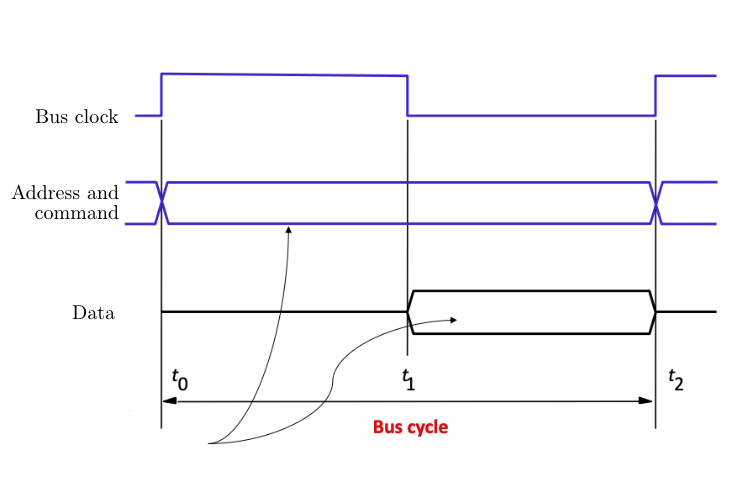
\includegraphics[width = 0.7\textwidth]{Images/Bus sincrono.png}
	\end{center}
	\caption{Bus sincrono}
\end{figure}
Nota come su ogni fronte basso il segnale viene spedito e rimane sul bus fino al prossimo fronte alto
\begin{itemize}
	\item Pro
	      \begin{itemize}
		      \item Molto semplice da implementare
		      \item Molto veloce
	      \end{itemize}
	\item Contro
	      \begin{itemize}
		      \item Poca robustezza alla variazione del clock (\textit{drift})
		      \item Tutte le periferiche sono vincolate alla velocità di clock
	      \end{itemize}
\end{itemize}
\subsubsection*{Bus asincroni}
Per ovviare ai problemi dei bus sincroni, spesso si ricorre all'uso dei bus asincroni
\begin{itemize}
	\item Non esiste un clock
	\item Le transazioni sono regolate da segnali \underline{handshake}
	\item Vengono introdotte linee di controllo per inizio e fine di transazioni
\end{itemize}
\begin{figure}[H]
	\begin{center}
		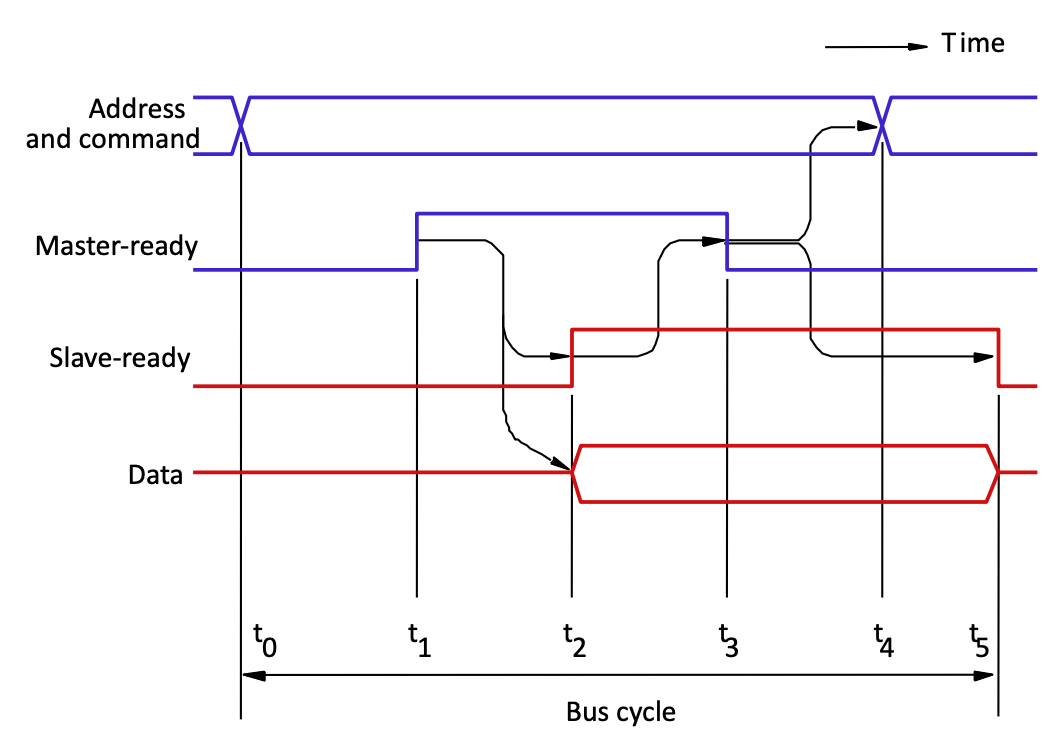
\includegraphics[width = 0.7\textwidth]{Images/Bus asincrono.png}
	\end{center}
	\caption{Bus sincrono}
\end{figure}
\begin{itemize}
	\item Il master (spesso il processore) manda un segnale allo slave (spesso memoria)
	\item Quando lo slave si setta a 1, il segnale viene retropropagato al master, che viene settato a 0
	\item Il dato rimane nel bus fino a quanto lo slave è settato a 1
\end{itemize}
Naturalmente, anche questa tecnologia prevede dei pro e dei contro
\begin{itemize}
	\item Pro
	      \begin{itemize}
		      \item Robusto rispetto al \textit{drift}
		      \item Comunica con periferiche di tipo diverso
	      \end{itemize}
	\item Contro
	      \begin{itemize}
		      \item Lento nelle interaioni
		      \item Cirtuiteria molto più complessa e costrosa
	      \end{itemize}
\end{itemize}
Per tale ragione spesso si usano tecnologie ibride, anche se \underline{prevalentemente asincrone}
\begin{center}
	\begin{tabular}{|m{0.2\textwidth}|m{0.2\textwidth}|m{0.2\textwidth}|m{0.2\textwidth}|}
		\hline
		Caratteristica                            & Firewire (1394) & USB 2.0                        & PCI Express              \\
		\hline
		Utilizzo previsto                         & Esterno         & Esterno                        & Interno                  \\[22pt]
		Numero disposiviti per canale 63          & 127             & 1                              & 1                        \\[22pt]
		Larghezza base dei dati                   & 4               & 2                              & 2 per linea              \\[22pt]
		Larghezza di banda picco teorica          & 50- 100 mb/s    & 0.2-1.5-60 mb/s                & 250 per linea            \\[22pt]
		Collegamento a caldo                      & Si              & Si                             & Dipende dalle dimensioni \\[22pt]
		Lunghezza massima del bus (piste in rame) & 4.5 metri       & 5 metri                        & 0.5 metri                \\[22pt]
		Nome dello standard                       & IEEE 1394       & Forum degli implementatori usb & SIG PCI                  \\[22pt]
		\hline
	\end{tabular}
	\vskip3mm
	\begin{tabular}{|c|c|c|}
		\hline
		Caratteristica                            & Serial ATA & Seria Attached SCSI \\
		\hline
		Utilizzo previsto                         & Interno    & Esterno             \\
		Numero disposiviti per canale 63          & 1          & 4                   \\
		Larghezza base dei dati                   & 4          & 4                   \\
		Larghezza di banda picco teorica          & 300 mb/s   & 300 mb/s            \\
		Collegamento a caldo                      & Si         & Si                  \\
		Lunghezza massima del bus (piste in rame) & 1 metro    & 8 metri             \\
		Nome dello standard                       & SATA-IO    & Comitato T10        \\
		\hline
	\end{tabular}
\end{center}
\subsubsection*{Esempio calcolatore a 32 bit}
\begin{figure}[H]
	\begin{center}
		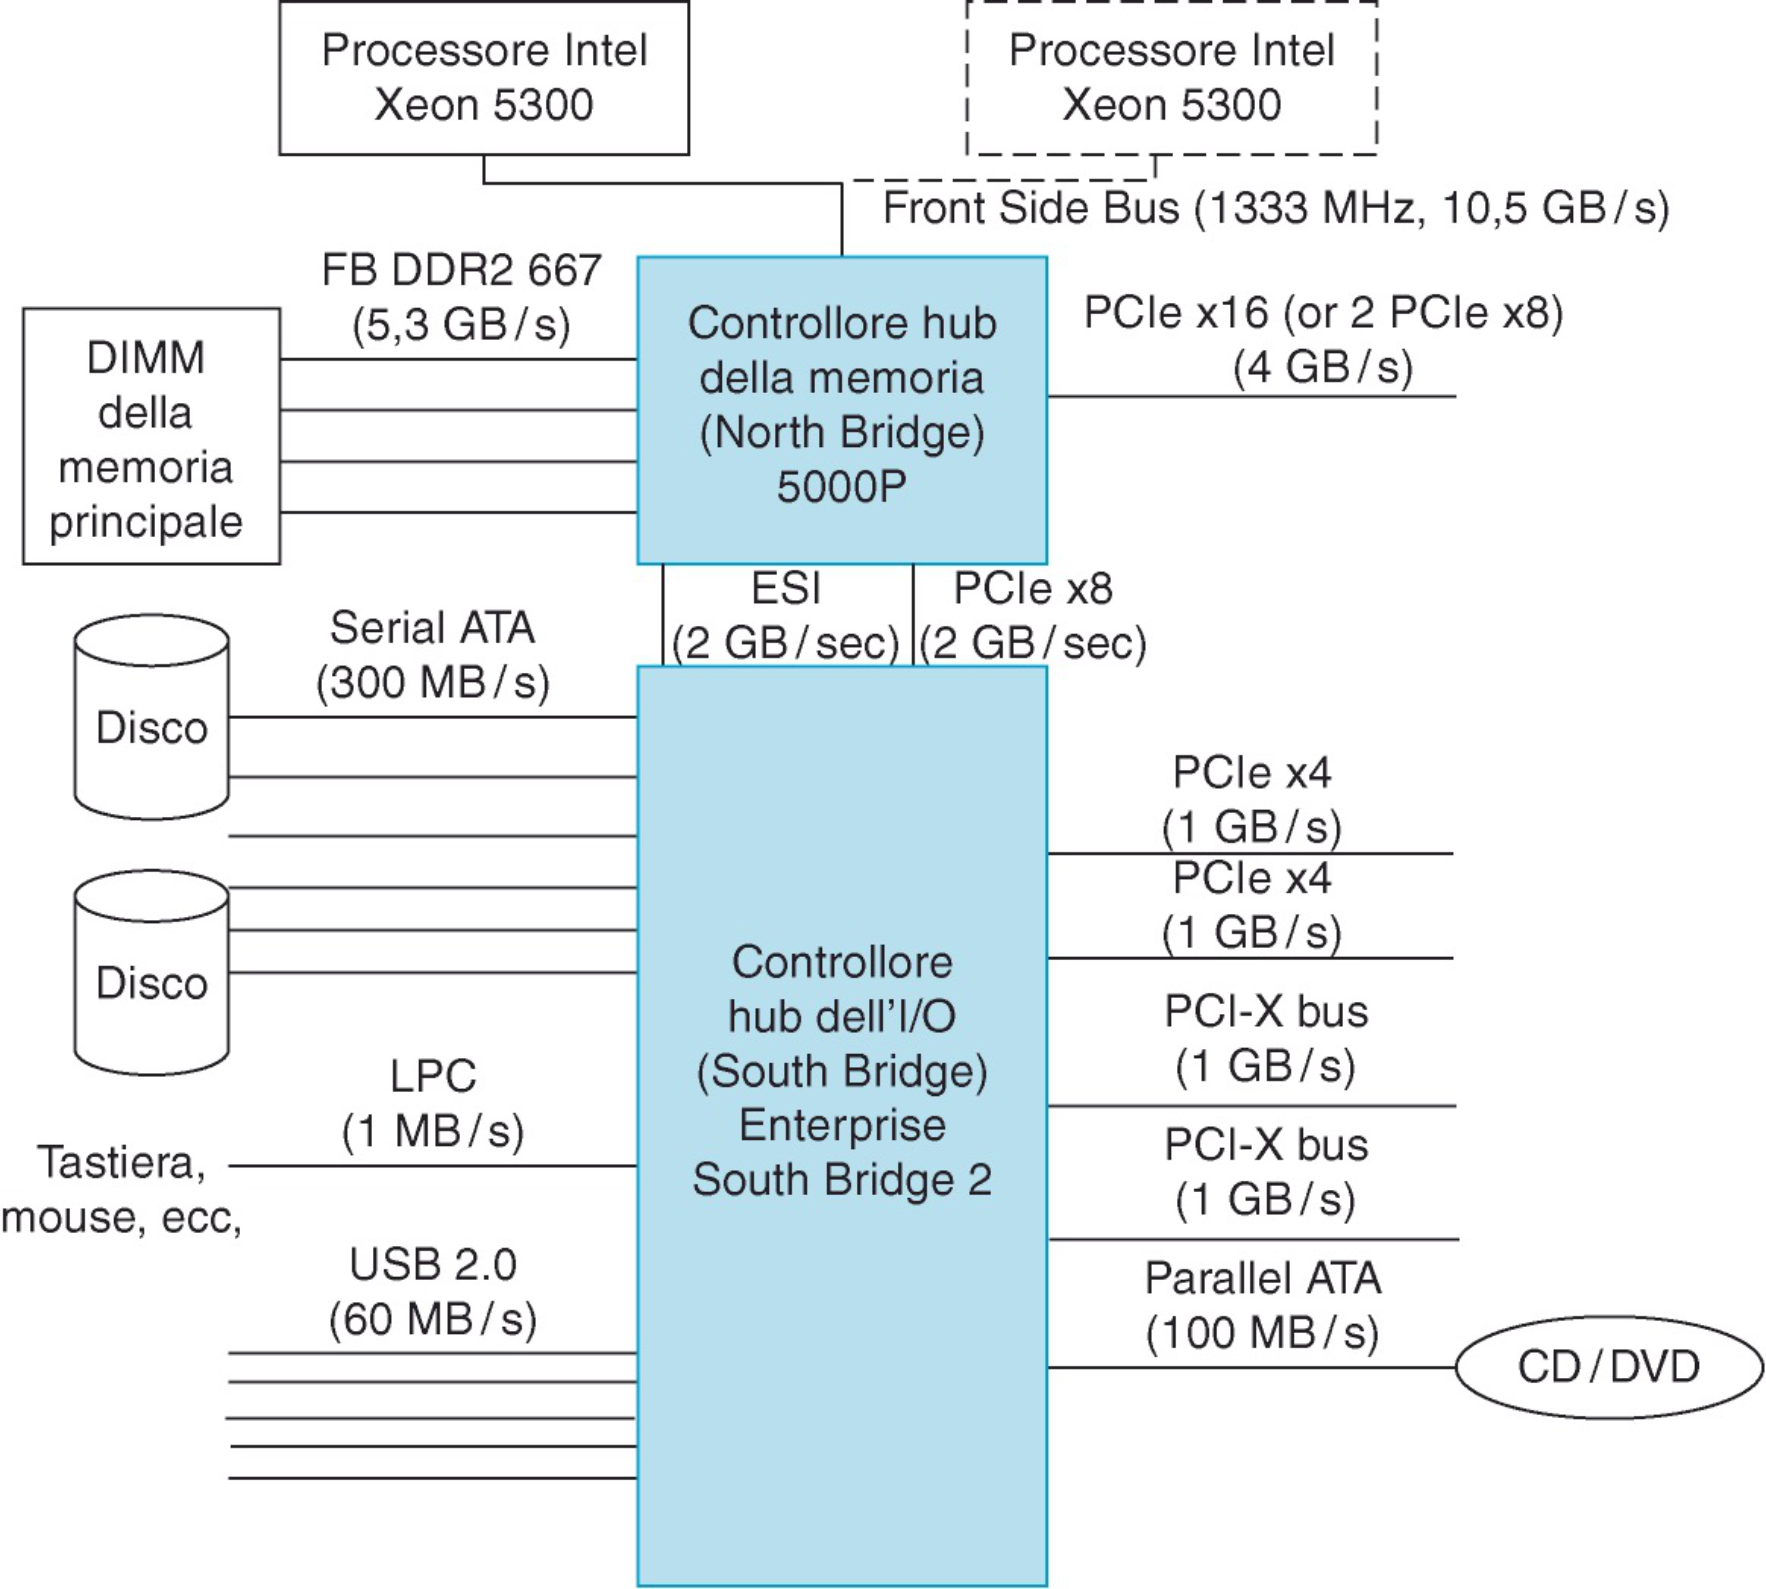
\includegraphics[width = 0.7\textwidth]{Images/Esempio x86.png }
	\end{center}
	\caption{Esempio x86}
\end{figure}
\subsection{Ruolo sistema operativo}
Il sistema operativo gestisce tutte le rischieste di input e output, in modo da garantire la collaborazione efficace da parte di tutte le prefiferiche. In particolare solo una parte del S.O. ossia il \underline{kernel}, interagiste in modalità protetta (\underline{modalità supervisor}) con il processore per gestire l'interazione fra le periferiche. Questa modalità si chiama \underline{modalità ad interrupt} (\textit{la periferica} manda un segnale che viene gestito dal kernel). Questa modalità serve per gestire i problemi di \underline{concorrenza} (ad esempio quando due programmi vogliono interagine con la stessa periferica)
\vskip3mm
il sistema operativo deve dunque implementare le seguenti funzionalità:
\begin{enumerate}
	\item Possibilità di inviare comandi alle \textit{periferiche}
	\item \textit{Le periferiche} devono poter notificare la corretta esecuzione di un'operazione, lanciando "eccezioni" nel caso vi siano errori
	\item Consentire trasferimenti diretti da dispositivo e memoria
\end{enumerate}
\subsubsection*{Memory mapped I/O}
La comunicazione alle periferiche può avvenire tramite la scrittura in determinate zone di memoria come segue:
\begin{itemize}
	\item Ogni dispositivo possiede area di memoria specifica (\underline{non accessibile al programmatore ma solo al S/O})
	\item Scrivendo su questa zona il \textit{controllore I/O} intercetta il segnale ed esegue il comando
\end{itemize}
Ad esempio, posso stampare su terminale tramite una system call e a stampa finita un preciso bit verrà settato ad 1 per indicare che la stampa è avvenuta correttamente
\vskip3mm
Per accertarmi che il comando sia avvenuta correttamente posso fare \underline{polling}, ossia continuo a "domandare" alla periferica se l'operazione è stata conclusa correttamente
\textbox{Il problema del polling è che il polling viene fatto \underline{sempre}, anche se l'operazione di I/O non viene eseguita}
\subsection{Interrupt}
Nel momento in cui l'attesa attiva(polling) risulta inaccettabile, (ad esempio nel caso di un disco rigido) si può utilizzare la modalità \underline{a interrupt}
\subsubsection*{Le eccezioni}
\textbox{In realtà un interrupt è un caso particolare di un evento del s.o.: \underline{le eccezioni}}
Vi sono due tipi di eccezioni:
\begin{itemize}
	\item \textit{Esterne}: ad esempio gli \underline{interrupt}
	\item \textit{Interne}: create dal programma stesso, ad esempio \textit{segmentation fault}
\end{itemize}
Le eccezioni avvengono durante l'esecuzione di un programma, e vengono gestite dal \underline{system exception handler}
\begin{itemize}
	\item Interrupts
	      \begin{itemize}
		      \item Causate da eventi esterni (I/O)
		      \item Asincrone
		      \item Sospendono il programma e ripendono da dove era stato interrotto
	      \end{itemize}
	\item Traps (eccezioni)
	      \begin{itemize}
		      \item Causate da eventi \textit{interni} al programma
		            \begin{itemize}
			            \item Condizioni eccezionali (\textit{arithmetic overflow, undefined instr})
			            \item Errori (\textit{hardware malfunction, segmentation fault})
			            \item Fault (\textit{non-resident page})
		            \end{itemize}
		      \item Sincrone
		      \item Gestite da \underline{trap halndler}
		      \item Possono causare l'aborto del programma
	      \end{itemize}
	\item Environment call/break
	      \begin{itemize}
		      \item All'interno del programma chiediamo esplicitamente di eseguire chiamate a sitema
		      \item Invocate ocn istruzione "\underline{ecall}", ad esempio la stampa di un carattere
		      \item Invocate tramite, ad esempio, l'aggiunta di un breakpoint tramite debugger (istruzione \textit{ebreak})
	      \end{itemize}
\end{itemize}
\subsubsection*{Gestione istruzioni}

\end{document}
